\chapter{High Voltage}
\label{ch:dp-hv}

%%%%%%%%%%%%%%%%%%%%%%%%%%%%%%%%%%%%%%%%%%%%%%%%%%%%%%%%%%%%%%%%%%%%
%\section{High Voltage System Overview}
\label{sec:fddp-hv-ov}

%%%%%%%%%%%%%%%%%%%%%%%%%%%%
%\subsection{Introduction - 2 pages}
\label{sec:fddp-hv-intro}

A \dword{lartpc} requires an equipotential cathode plane at \dword{hv} and a precisely regulated interior \efield to drive 
electrons from particle interactions to sensor planes.  For the \dword{dune} \dlong{dp} (\dword{dp}) technology, 
this requires a horizontal cathode plane, held at negative \dword{hv}; a horizontal charge readout plane (CRP) in the gas phase as described in Chapter~\ref{sec:fddp-crp-intro}; and formed sets of conductors at graded voltages surrounding the
 the central drift volume, collectively called the \dword{fc}, shown in Figure~\ref{fig:dune_dp_fd_hvs}. The \dword{fc} consists of electrically and mechanically continuous, field shaping rings that provide voltage degradation in the vertical direction; it forms one continuous active volume.


\begin{dunefigure}[\Dword{dpmod} overview]{fig:dune_dp_fd_hvs}
{An isometric view of the DP HV system components. Most of the \dword{fc} profiles are removed to emphasize the structural elements.  The figure shows 3 completed \dword{fc} super-modules on the upper right, the structural members of the \dword{fc} and cathode plane in the lower left, and half the ground grid modules on the bottom.  The entire structure is suspended under the cryostat ceiling by 24 cables/rods (Credit: BNL) }.
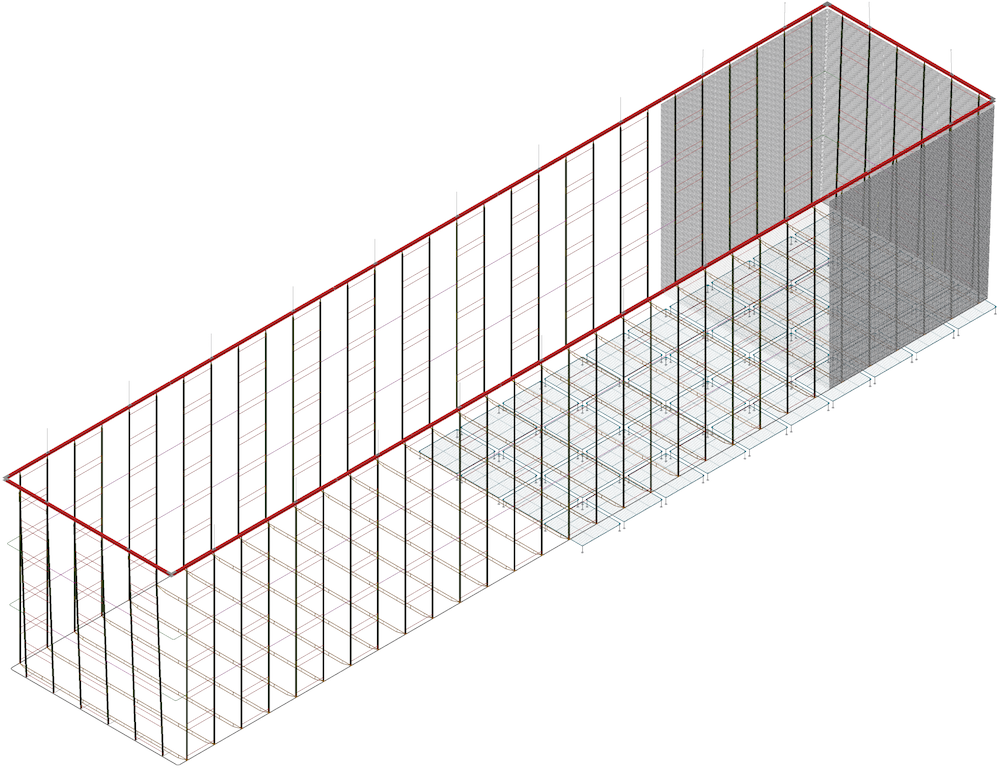
\includegraphics[width=0.9\textwidth]{DP_HVS_v1.png}
\end{dunefigure}

The \dword{hv} consortium will provide a system that operates at the nominal voltage corresponding to the uniform \SI{500}{V/cm} \efield in the \dword{tpc} drift volume. As a result, its systems %actually 
constitute a large fraction of the %total 
internal structures of the \dword{tpc}. % itself. 
Mechanical and structural concerns are taken into account, together with the electrical design to meet the requirements. 

The scope of the \dual \dword{hv} system, provided by the \dword{dune} \dword{hv} consortium includes selecting and procuring materials, as well as the fabrication, testing, delivery, and installation of the systems needed to generate, distribute, and regulate the voltages that
create a stable and precise \efield{} within a \dword{dpmod}. 

The \dword{hv} system consists of components both exterior and interior to the cryostat. The voltage generated at the \dword{hv} power supplies passes through the cables, filters, and the \dword{hv} \fdth into the cryostat. From the point of delivery into the cryostat, components that form part of the \dword{tpc} structure further distribute the voltage. The internal \dword{hv} components, in fact, form a large fraction of the total internal structure of the \dword{tpc} itself, and  
 %largely 
 effectively bound the fiducial volume of the %experiment 
 \dword{detmodule}. The \dword{hv} system is a key to determining the event rate for all \dword{dune} physics processes.

The \dword{hv} system consists of
\begin{itemize}
\item \dword{hv} power supplies, cables, filters, and feedthroughs;
\item  a horizontal cathode (about \SI{60}{\m} long and \SI{12}{\m} wide) made of arrays of resistive elements placed about \SI{1.5}{\m} above the bottom of the cryostat;
\item vertical \dword{fc} walls, \SI{12}{\m} tall surrounding the cathode;
\item \dwords{gp} below the cathode to protect the Photon Detector array.
\end{itemize}

The system operates at the full range of voltages, %all voltages, from the highest 
%maximum 
$-$\dptargetdriftvoltpos to ground, inside the \dword{tpc} volume. 

The \single and \dual modules will use similar designs for some
 \dword{hv} system components, %including the \dwords{fc} profiles and supporting FRP beams, and the voltage divider boards. More details can be found in   
in particular, aspects of the \dwords{fc} and its supporting beams. The dual phase versions are described in this chapter. 
 %\fixme{for Anne  let's list sections where these components are described. Anne}.

The design presented in this chapter is primarily based on the \dword{pddp}, \dword{pdsp}, and \dword{wa105} \fixme{This is not in the common glossary, so something is missing in the PDF.} experience. 


%%%%%%%%%%%%%%%%%%%%%%%%%%%%%%%%%%%%%

%%%%%%%%%%%%%%%%%%%%%%%%%%%%
\subsection{Design Requirements -3 pages}
\label{sec:fddp-hv-des-consid}

The working principle of the \dword{lartpc} relies on applying a very uniform strong \efield in ultra-pure liquid argon.  A number of detector performance parameters benefit from such an \efield in ways that directly support the core components of the \dword{dune} physics program.  Some of these are examined in detail in Volume 2, the Physics \dword{tdr}.  Here we set the context by presenting a qualitative description of \efield effects on physics.

Because free electron drift velocity in \dword{lar} is a function of \efield, a uniform \efield allows mapping along the drift direction using simple time versus position and enabling precise and efficient \threed reconstruction.  This allows, for example, establishing a well defined fiducial volume for beam neutrino events reconstructed in the Far Detector.  A neutrino \dword{cp} violation measurement, or mass hierarchy test, at root compares normalized spectra for electron and muon neutrino and antineutrino interactions in the fiducial volume of the Far Detector, as projected from the Near Detector; for this reason, fiducial volume characterization is critical.   

Spectral information is necessary to separate \dword{cp} and mass hierarchy effects, necessitating efficient tracking and shower reconstruction and good energy resolution. Toward these ends, higher \efield strengths are generally better.  More free charge is created at the ionization points because recombination decreases at higher fields, improving signal-to-noise and calorimetry. Drift times are reduced, resulting in less electron capture and better signal-to-noise, even under less than optimal purity conditions.  Spatial resolution improves as $\sqrt{t_{drift}}$ dependent diffusion effects lessen. Higher free charge production and lower electron capture gives lower detection thresholds on components of electromagnetic showers, improving shower energy reconstruction.  Lower detection thresholds also lead to higher detection efficiency for MeV-scale electron, photon, and neutron signatures of low energy $\nu_e$ interactions from supernova neutrino burst events.  The decreased recombination affects highly ionizing particles, usually protons, more than minimum ionizing particles. Less saturation of free charge production occurs, leading to better particle identification and more precise energy measurements. Lower recombination particularly helps proton-kaon separation by $dEdx$, a key component of a search for $p\rightarrow K^+ \nu$ baryon decay events. 

However, apart from obvious technical limitations, the \efield should not be raised beyond certain limits. For instance, while free charge production increases with \efield, scintillation photon production decreases, resulting in fewer photons available for triggering and T=0 purposes. Two-track separation can degrade, if drift velocity is increased while keeping anode wire separation and electronic wave form sampling fixed. The distance between the \dword{tpc} boundaries and the cryostat walls would likely need to be increased for very high \efield{}s to prevent electrostatic discharge. This would, in turn, reduce the fraction of liquid argon in the fiducial volume. The effects of the first is modest, and all effects are subsumed by technical challenges in delivering high voltage to the cryostat and maintaining highly stable high voltage surfaces for several decades of operation. These challenges require developing non-commercial cryogenic \dword{hv} feedthroughs, \dword{hv} ripple-repression through custom \dword{hv} \dword{rc} circuits, careful construction and deployment of \dword{hv} cables, redundant \dword{hv} connections, high quality monitoring, and best practices at all stages of design, installation, and operation.

Two decades of design and operational experience that began with ICARUS have established that a 500 V/cm field is an appropriate trade-off value that can be realistically achieved using cost-effective design and construction methods. Achieving this design goal will be challenging because the drift distance has progressively increased to the \SI{12}{m} foreseen for the \dword{dpmod}, and overall detector optimization has proved important. 
The forthcoming test of \dword{protodune} NP02 will likely run at the nominal \dword{hv} of \SI{-300}{kV}.\  Its successful operation will confirm that \dword{dune} \dword{dp} can operate  at least at E=250 V/cm.
However, DUNE must be able to run at higher voltage, up to the nominal 500 V/cm, to compensate for unexpectedly low purity conditions that could arise over two decades of planned operation.
%For example, MicroBooNE operates  at 273 V/cm (lower that its nominal value of 500 V/cm), and is able to operate well by exploiting its very high argon purity, (characterized by an electron lifetime in excess of 15 ms), as well as an excellent signal-to noise ratio from the front end cold electronics.  %The latter allows hit identification even for signals attenuated by diffusion and lifetime. 
%due to the larger electron diffusion and the finite lifetime,
%MicroBooNE (and a number of other liquid noble TPCs) compensated for electrostatic instability problems by achieving higher purity, and DUNE might well operate in this mode during its run.  Ω

%\fixme{(It would be better if we could cite ProtoDUNE)} 
The 500 V/cm \efield goal, combined with high \dword{lar} purity, a large signal-to-noise ratio, and a large CRT gain, will allow  a wide range of possible operating points to optimize detector performance for maximum physics potential over decades of stable conditions and very high live time. 
%\fixme{some duplications in the paragraph above and below - BY}
The specifications for the \dword{dune} \dword{dp} \dword{hv} system thus have the goal of 500 V/cm, pointed  toward the highest possible detector performance and widest span of operating points, and a minimum of 250 V/cm, which would provide minimal detector performance, assuming achievable purity and electronics parameters. 

Unlike the \dword{sp} case, in the \dword{dp} detector, space charge could be non negligible in distorting the electric field uniformity because of the presence of the irreducible Ar39 radioactive background that constantly produces positive ions in \dword{lar} and the long drift distance that prolongs their permanence in the drift volume. In addition, this effect could be highly enhanced by the injections into \dword{lar} of the positive ions produced by the electron multiplication in the CRT amplification stage (up to a factor 20 at nominal CRT gain). To mitigate this effect, the electric field in the drift region must be as high as possible, which allows speediing up positive ions in \dword{lar} toward the cathode where they are neutralized, thus reducing the overall space charge. Hence, the goal of reaching the nominal value of 500 V/cm is much more important for the \dword{dp} case, in spite of the higher technological challenge of applying -600 kV on the cathode. 

The \dword{hv} system is designed to meet the physics requirements of the \dword{dune} experiment. This includes both physical requirements (e.g., an \efield 
that allows robust event reconstruction) and operational requirements (e.g., 
avoiding over-complication to maximize data collection efficiency). 
A collection of essential requirements for the \dword{hv} system is shown in Table~\ref{tab:hvphysicsreqs}.

\begin{dunetable}
[\Dword{hv} system requirements]{p{0.05\textwidth}p{0.2\textwidth}p{0.35\textwidth}p{0.15\textwidth}p{0.15\textwidth}}
{tab:hvphysicsreqs}
{\dword{hv} System Requirements.}
No. & Requirement & Physics requirement driver & Requirement & Goal \\ \toprowrule
1 & Exceed minimum \efield TPC drift volume & Maintain adequate particle ID, which is affected by slower drift speed and increased recombination, diffusion, and space charge. & >\SI{250}{V/cm} &\SI{500}{V/cm} \\ \colhline
 2 & Do not exceed maximum \efield in \lar volume & Avoid damage to detector to enable data collection over long periods. & \SI{30}{kV/cm} & \dword{alara} \\  \colhline
3 & Minimize power supply ripple & Keep readout electronics free from external noise. %, which confuses event reconstruction.  
\\ \colhline
4 &  Maximize power supply stability & Maintain the ability to reconstruct data taken over long periods.  Maintain high operational up time to maximize experimental statistics. \\ \colhline
5 & Provide adequate decay time constant for discharge of the cathode plane and \dword{fc} as well as cathode plane resistive segmentation & Avoid damage to detector to enable data collection over long periods. Maintain high operational up time to maximize experimental statistics. & \si{\giga\ohm} resistors per each connection of the $3\times3$m$_2$ cathode units  \\ \colhline
6 & Provide redundancy in all \dword{hv} connections & Avoid single-point failures in detector that interrupt data taking. & > 2 voltage divider chains to distribute \dword{hv} to the \dword{fc} profiles & one voltage divider chain every four \dword{fc} modules\\ 
\end{dunetable}

%%%%%%%%%%%%%%%%%%%%%%%%%%%%
\subsection{Scope }
\label{sec:fddp-hv-scope}

The scope of the \dword{hv} system 
includes procuring materials and the fabricating, testing, delivering and installing the components of the system that generates, distributes, and regulates voltages to create a precision \efield within the \detmodule volume. 

The \dword{hv} system consists of components both exterior and interior to the cryostat. The \dword{hv} power supply is external to the cryostat.  In the \dword{dpmod}, the \dword{hv} power supply should be on top of the \dword{hv} \fdth. \Dword{hv} is further distributed by interior components that form part of the \dword{tpc} structure. Figure~\ref{fig:dune-dp-hvs} a shows the schematic overview of the \dword{hv} system (panels b-d show pictures of some related components from \dword{wa105}).

The \dual \dword{hv} system has the following components:

\begin{itemize}
\item \SI{-600}{kV} \  power supply,
\item \dword{hv} \fdth,
\item \dword{hv} extender and voltage degrader,
\item Cathode plane and \dword{gp}, 
\item Field cage, and
\item \dword{hv} return \fdth and resistor box.
\end{itemize}

\begin{dunefigure}[HV system for a \dpmod ]
{fig:dune-dp-hvs}
{(a) Schematic overview of the \dword{hv} system for a \dpmod{}, 
(b) photograph of the \SI{300}{\kV} Heinzinger power supply\footnote{Heinzinger\texttrademark{} PNChp 300000 power supply.}, (c) the VHV \fdth{}, and (d) the \dword{hv} return connection. (All photographs from \dword{wa105}.)}
%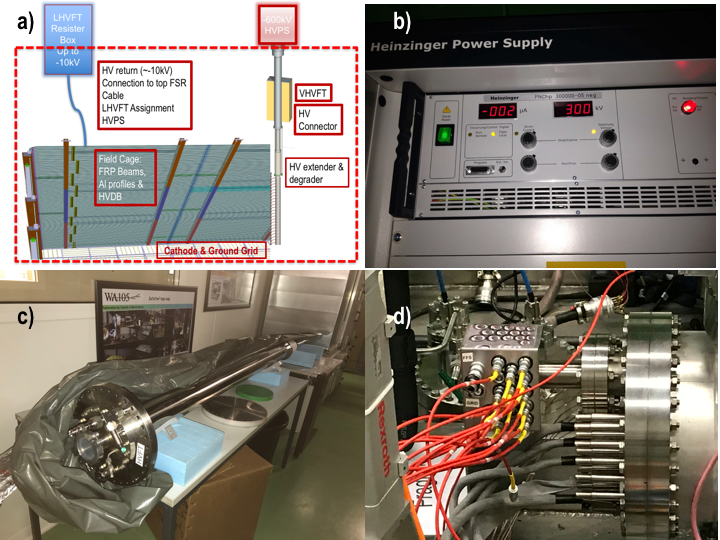
\includegraphics[width=1.0\textwidth,height=1.2\textwidth]{graphics/dp-hvs-n-photos.png}
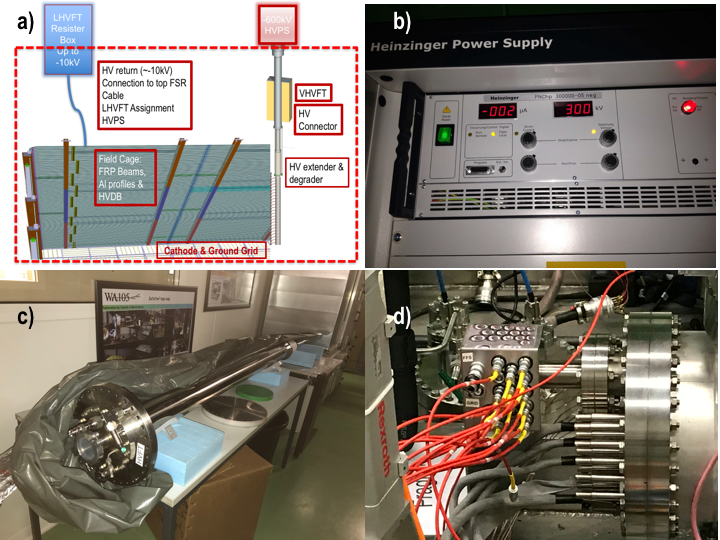
\includegraphics[width=0.8\textwidth]{DP_HVS_dp-hvs-n-photos.png}
\end{dunefigure}


\clearpage
%%%%%%%%%%%%%%%%%%%%%%%%%%%%%%%%%%%%%%%%%%%%%%%%%%%%%%%%%%%%%%%%%%%%
\section{ProtoDUNE Experience}
\label{sec:fddp-hv-protodune}
%\subsection{Summary of Construction and Operation - 1 page }
\label{sec:fddp-hv-protodune-summary}
%%%%%%%%%%%%%%%%%%%%%%%%%%%%

The \dword{pddp} detector was designed to cover \SI{6}{\m} x \SI{6}{\m} x \SI{6}{\m} active volume.
This enabled testing the concept of scalable final detector components, in particular the \dword{crp}, the cathode, and the \dword{gp} whose unit component dimensions are \SI{3}{\m} (W) $\times$ \SI{3}{\m} (L).
The \dword{fc} of the \dword{pddp} covered the \SI{6}{\m} $\times$ \SI{6}{\m} $\times$ \SI{6}{\m} active volume, so the testing was effectively done using the concept that each of the sub-modules make the \dword{fc} module of dimension \SI{3}{\m} (W) $\times$ \SI{6}{\m} (H).
The VHV applied to the cathode was at maximum \SI{-300}{\kV} to provide a \SI{500}{\V/\cm} drift field.
The sub-module assembly procedure and the subsequent installation procedure were tested in the cryostat and can be applied to \dword{dune} with some minor changes to reflect the lessons learned from \dword{pddp} installation. 

\begin{dunefigure}[\dual \dword{hvdb}]{fig:dp-hvdb}{\dword{pddp} \dword{hv} divider board: (a) schematic circuit diagram, (b) photograph of the top of the board, and (c) photograph of the bottom of the board.}
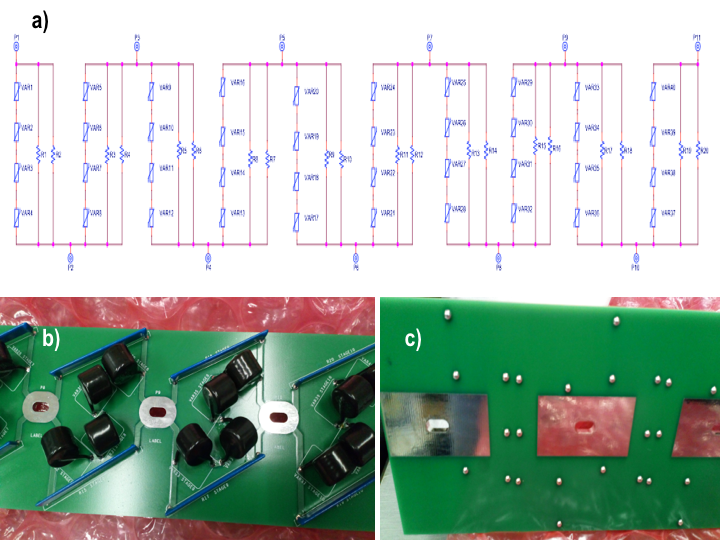
\includegraphics[width=0.75\textwidth]{DP_HVS_dp-hvdb.png}
\end{dunefigure}

\subsection{Design}
\label{sec:fddp-hv-protodune-lessons-design}
The design of the \dword{pddp} \dword{fc} sub-modules used two \SI{15.2}{\cm} (\SI{6}\,in) FRP frames connected by two \SI{7.6}{\cm} (\SI{3}\,in) FRP cross bars, to form a frame. 
The two \SI{15.2}{\cm} (\SI{6}\,in) FRP frames had slots conforming to the shape of the aluminum profiles in which to insert them.
Because the mechanical connections between the sub-modules use 10cm wide G10 plates, a large number of insulators from the FRP frames are exposed toward the cryostat membrane wall at ground.
The design of the \dword{fc} sub-module has been changed to minimize insulator exposure toward the cryostat membrane wall because unexpected streamers were observed in \dword{pdsp} operations.  
Now, the new design for \dword{dune} has no insulators exposed toward the wall, leaving all inter-sub-module mechanical connections inside the active volume, away from the walls.
To reduce the drift field distortion from surface charging, the cross bars are replaced with stainless steel tubes as described in detail below.

In \dword{pddp}, the aluminum profile electrodes are interconnected to form an electrically continuous field shaping ring, using metal clips that conform to the shape of the profile.  
The cathode is also designed to be constructed out of stainless steel tubes. 
These two design concepts raised significant concerns about the possibility of a large amount of stored energy discharging toward the membrane wall or the floor and seriously damaging the cryostat wall. This would virtually disable detector operations and cause a significant safety hazard.
To address these safety concerns, in \dword{dune} \dword{dp} the metal profile clips are replaced with resistive sheaths, and the cathode modules are now made of resistive tubes held by metal trusses as described below.

Two types of resistive VHV divider boards as shown in Figure~\ref{fig:pddp-hvdb} are designed to cover \num{9} and \num{8} gaps, respectively.
\fixme{This is not entirely clear because the two types of resistive VHV divider boards are not named. In addition, pairing up the divider boards with the respective gaps would be clearer than using the phrasing necessary to "respectively."  Resistive VHV divider board X is designed to cover \num{9} gaps, and resistive VHV divider board Y is designed to cover \num{8} gaps. See Figure~\ref{fig:pddp-hvdb}.}
Ample redundancy has been built into the board design, so each gap has two \SI{2}{\giga\ohm} main resistors and four varistors to accommodate up to \SI{6}{\kV}, twice the operation voltage in case the final \SI{600}{\kV} VHV power supply becomes available.
An additional row of \dword{hvdb} was installed in the \dword{fc} for additional redundancy, taking advantage of the electrically continuous field shaping rings.
The board design will change slightly for \dword{dune} to minimize the potential for a discharge between the back of the board and the field shaping profiles and to reduce the number of varistors to cover the \SI{3}{\kV} operational potential difference between the two adjacent profiles.

\begin{dunefigure}[\dual \dword{hvdb}]{fig:pddp-hvdb}{\dword{pddp} \dword{hv} divider board (a) schematic circuit diagram, (b)photo of the top of the board, (c) photo of the bottom of the board}
%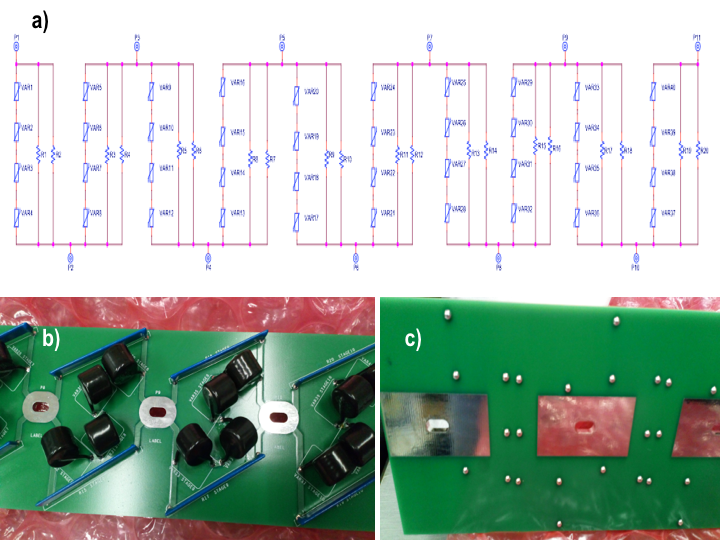
\includegraphics[width=0.75\textwidth]{graphics/dp-hvdb.png}
\end{dunefigure}
\fixme{(anne) this figure is referenced in several places but whole figure was commented out. Figure out what to do about figure.}

\subsection{Construction}
\label{sec:fddp-hv-protodune-lessons-construction}
The FRP parts for the \dword{fc} are processed at the factory to eliminate burrs and defects left on the parts for quality control and quality assurance.  
These parts are then cleaned following a procedure using de-ionized water and then dried in a humidity controlled storage room.
Once the parts are sufficiently dried, the processed surface areas are covered with polyurethane varnish for further protection.
The parts are then brought to a humidity controlled cleanroom (class ~10,000), put together as a frame to ensure mechanical fitness, disassembled and packaged as a compact package of \SI{0.2}{\m} (W) $\times$ \SI{0.2}{\m} (H) $\times$ \SI{2}{\m} (L) and wrapped in plastic shrink wrap for storage before shipment.
This process worked out well in \dword{pddp}, so the same process will be followed in \dword{dune} \dual as well.
The design change makes it easier to process and condition FRP parts.
In addition, the size of the package for each sub-module will be considerably more compact than the \dword{pddp} \dword{fc} sub-modules.

\begin{dunefigure}[\dword{fc} parts]{fig:dune-dp-fc-all}
{\dword{fc} parts and connections for \dword{pddp}:  a. One \dword{pddp} \dword{fc} panel consisting of three sub-modules.  The \dword{dpmod} has a virtually identical structure except for the number of middle sub-modules (four) and the profile lengths (4m instead of the 3m) in \dword{pddp}; b. A photograph of the top module connection to the stainless steel I-beam and an inter-sub-module connection; c. Aluminum clip connection at the corner and at the straight sections.  These clips will be replaced with a resistive sheath in \dword{dpmod}; d. \dword{hv} divider boards and their connections on \dword{pddp} \dword{fc}. }
%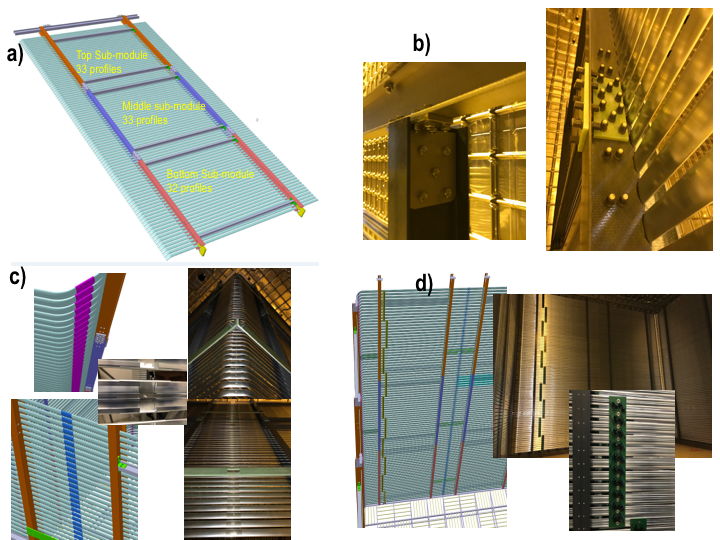
\includegraphics[width=1.0\textwidth,height=1.0\textwidth]{graphics/dp-fc-parts.png}
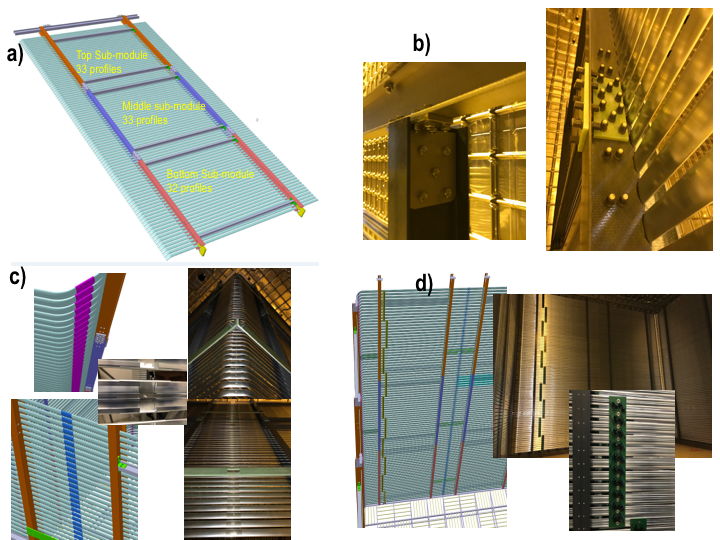
\includegraphics[width=0.9\textwidth]{DP_HVS_dp-fc-parts.png}
\end{dunefigure}

The resistor and varistor parts for the VHV divider boards are tested in air while warm, in liquid nitrogen for cold, and then again in air after warm up, to ensure the quality and resilience of the parts.  
Based on these measurements, parts are selected to ensure resistance values are within \num{1}~\% \fixme{There is an extra space between the number and the percent marking in the PDF. That space should be removed.} of the mean. 
The parts are then shipped to the contractor to be mounted on the printed circuit board with through holes allowing soldering on the back of the board.
The boards with resistors mounted on them are then tested again for quality assurance, twice in air and once in LN2, unless any of the gaps fail the quality control criteria.
The same quality control process will be used for \dword{dune} \dual as well.

The cathode units are built out of stainless steel tubes welded together in a structure that gives sufficient light transparency.
To slow down energy release from an unexpected discharge in \dword{pddp}, resistor boards are built to inter-connect two neighboring cathode units.
This resistor network, however, affected the input voltage to the \dword{hvdb} row diagonally across the \dword{fc} panel that accepts VHVPS input. The bottom most gap of the \dword{hvdb} row was then modified to compensate for the voltage drop across the diagonal distance from the VHV input.
This choice to implement resistors, and thus slow down energy release, has been taken into account in \dword{dune} \dual cathode design, as described below.

\subsection{Assembly and Installation}
\label{sec:fddp-hv-protodune-lessons-assy}
The \dword{fc} sub-modules were built in the cleanroom buffer in front of the \dword{tco} of the \dword{pddp} cryostat.
The assembly of each sub-module, including inserting and securing the profiles onto the FRP frame takes two people approximately two hours.
When as many sub-modules are built as the cleanroom buffer storage space allows, they are brought into the cryostat for installation.
Installing each \SI{6}{\m} (H) $\times$ \SI{3}{\m} (W) full length module begins with hanging the top sub-module to a $\sim$ \SI{3}{\m} stainless steel I-beam attached to the stainless steel cable through the ceiling.
The subsequent two sub-modules are then hung onto the top module successively.
The whole installation process for a \SI{6}{\m} module takes four people approximately an hour with
two people inside the cryostat connecting the modules while the other two are outside, on top of the cryostat roof, operating the winches that raise the corresponding partial module as successive sub-modules are attached.
This scheme requires two \fdth holes per module, which makes the total number of \fdth holes too large.

\begin{dunefigure}[\dual \dword{fc} installation process and inter-module connection]{fig:dp-fc-installation-connection}{Left: Two sub-modules connected and hanging from the two sets of stainless steel cables on the ceiling.  The lifting wires raise the module to its position as sub-modules are connected; the hanging wires keep the fully integrated module in its final position.  Right: Inter-sub-module connections.  Each connection is made with two \SI{1}{cm} thick G10 plates along the height of the I-beams and one \SI{1}{cm} thick G10 plate on the flange.}
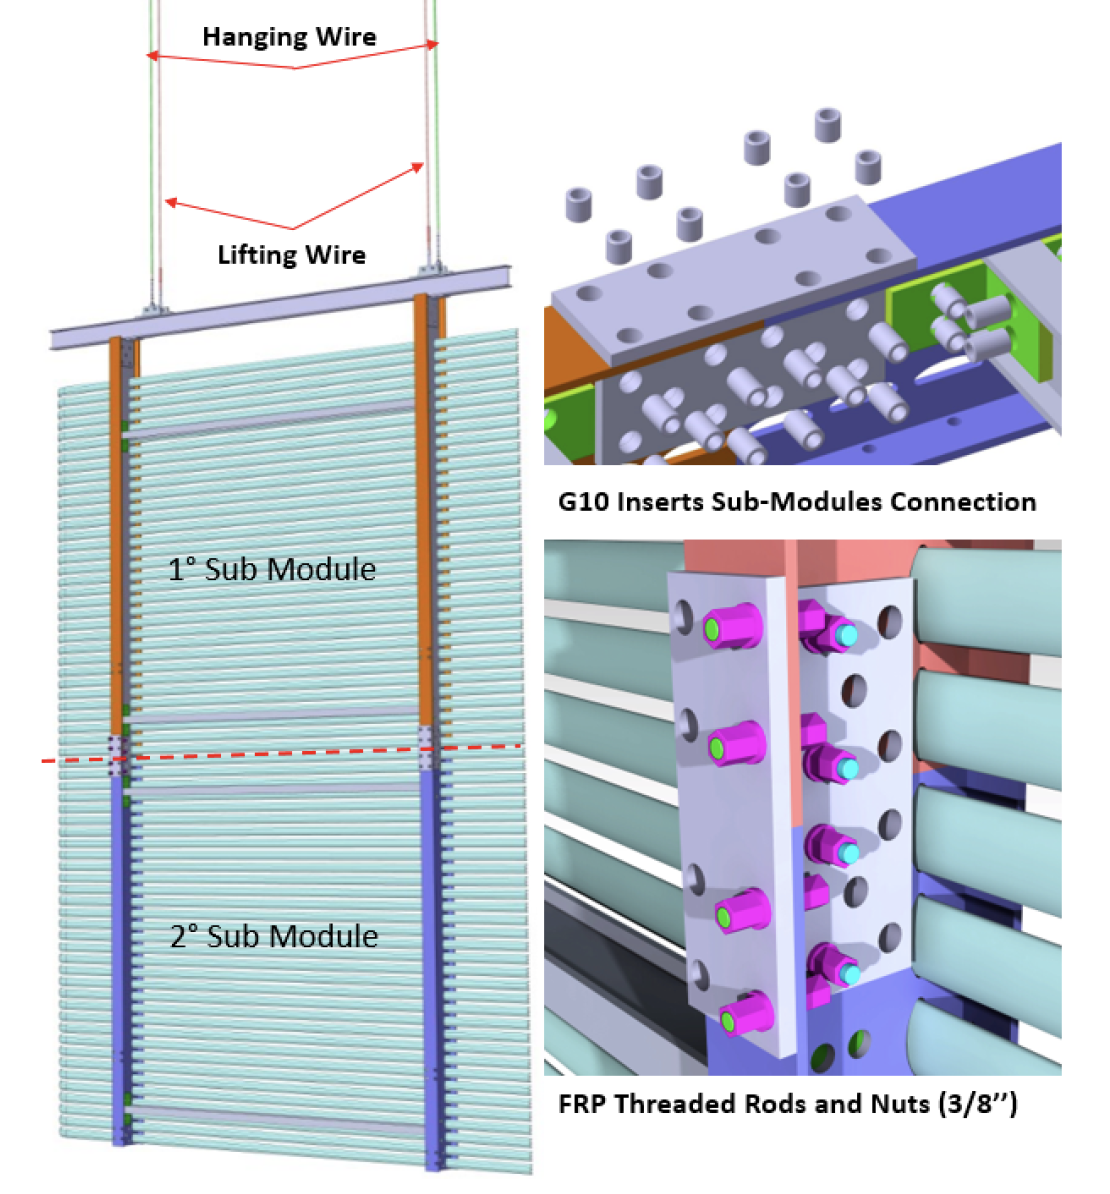
\includegraphics[width=0.75\textwidth]{DP_HVS_module-connection-installation.png}
\end{dunefigure}

A modified installation plan has been developed to dramatically reduce the number of \fdth holes and reduce the parts needed for the \dword{fc} modules as described below.

The \SI{3}{\m} (L) $\times$ \SI{3}{\m} (W) cathode and \dword{gg} modules are preassembled outside of the cleanroom buffer and brought into the cryostat for installation.
The assembly and installation scheme for the \dword{dune} \dword{dp} cathode must also change because its structure and the material composition will be modified to increase dramatically the time for energy release with the final goal of protecting the cryostat.

\subsection{Performance}
\label{sec:fddp-hv-protodune-lessons-perf}

The \dword{pddp} detector is not yet in operation at the time of this writing, so we can provide no input on performance other than the air commissioning we have performed and summarized in the previous sections.
%%%%%%%%%%%%%%%%%%%%%%%%%%%%

\subsection{Lessons from ProtoDUNE - 3 pages}
\label{sec:fddp-hv-protodune-lessons}
To ensure the performance of the \dword{fc} and to identify any issues well before the final installation of the detector pieces, the \dword{fc} unit has been connected to a \SI{150}{\kV} power supply.
For this air commissioning test, the entire field cage has been fully installed and connected using slip nuts for inter-module connections for electrical continuity.
As connections were made to each of the field shaping ring, the resistance between the two neighboring rings was measured and compared to expected values.
The \SI{150}{\kV} \dword{hv} was fed into the two middle field shaping rings along the field cage. This ensures a voltage difference between any two neighboring rings of \SI{3}{\kV} (which is the operational value) when the top most and bottom most rings are connected to the ground on the membrane wall.

An online wide angle camera was placed on the floor at the corner where the \dword{hv} fed in to ensure any possible sparks could be seen.
Current and voltage were carefully monitored and recorded to make sure any discharges could be observed and studied.
When the \dword{hv} was turned on for the first time, we observed the current settled after a charge up was approximately \num{50}~\% higher than expected.
Voltage was left on for many hours so we could observe the long term behavior.
The current continually increased to unexpectedly higher values several times while the testing was done, i.e., multiple power cycles.
A systematic test revealed that the size of the current read back was directly proportional to the number of \dword{fc} modules.

This test pointed in the direction of the FRP beams, leading to the assumption that ambient humidity allowed a layer of water to cover the surface, so the current flowed through the water layer.
Resistance measurements of a \SI{50}{\cm} long \SI{15.2}{\cm} (\SI{6}{in}) wide I-beam sample piece in air with similar humidity and in \dword{lar} showed that while the current in air is consistent with what was observed for \dword{pddp} \dword{fc}, and once the FRP I-beam is in the liquid, the resistance showed expected values with virtually no surface current flowing through.
Because this behavior was not observed in \dword{pdsp} \dword{fc}, we suspect that the FRP beams from a different manufacturer may have different surface water adhesion behaviors. It may be necessary to study the FRP beam from the current manufacturer in further detail for \dual \dword{fc}.


\subsection{Suggestions for future R\&D - 1 page}
\label{sec:fddp-hv-protodune-RD}
Per experiences from construction, assembly, installation and the "air commissioning" of the high voltage system at \dword{pddp}, the following R\&D items have been identified.

\begin{itemize}
    \item FRP surface water adhesion property,
    \item Resistive sheath,
    \item Distance between the two neighboring profiles,
    \item Optimal resistance for delaying energy releases. 
\end{itemize}
\clearpage

%%%%%%%%%%%%%%%%%%%%%%%%%%%%%%%%%%%%%%%%%%%%%%%%%%%%%%%%%%%%%%%%%%%%

\section{HV System Design}
\label{sec:fddp-hv-design}

%\subsection{Design Considerations}

Among the design considerations are many challenges scaling the \dword{pddp} \dword{tpc} design to the \dword{dune} \dword{fd}. The most prominent ones are 
\begin{itemize}
    \item Generating and transmitting the \SI{600}{\kV} voltage safely to the cathode plane 12m below the liquid level.
    \item Safely dissipating the energy stored ($\sim$ \SI{3}{\kJ}) in the entire \dword{tpc} in the event of a \dword{hv} discharge.
    \item Managing the different thermal contraction rate from different materials over the 60m length of the \dword{tpc}.
\end{itemize}

Generating and transmitting \SI{600}{\kV} to the cathode remain an R\&D item in collaboration with Heinzinger.

For the \dual \dword{fd} HVS, we are adopting the concept developed in the \single \dword{tpc} \dword{hv} system design, where the \dword{fc} modules are electrically isolated from each other, and the cathode is made entirely of highly resistive panels.  The implementations for the \dword{fc} and cathode are summarized as follows:
    
The basic \dword{fc} sub-modules are \SI{2}{\m} high and \SI{4}{\m} wide, We must stack \num{6} such sub-modules for a full module covering the \SI{12}{\m} drift length. Three such modules form a super-module \fixme{Please don't use SM as an abbreviation for super-module. SM is already in the glossary and stands for standard model.} and are suspended under one stainless steel beam.  On the middle module, along the vertical direction, the \dword{fc} profiles are interconnected with \SI{1}{\giga\ohm} resistance and parallel to surge suppressors to protect the resistors. The top and bottom module profiles are resistively coupled to the center module profile of the same height, reaching the same bias voltage because no current flows across the modules.  Similar resistive interconnects are also made between the profiles across super-modules to provide additional redundancy between super-modules.

The basic mechanical and electrical element of the cathode plane is a \SI{12}{\m} long metal truss structure connecting the two opposing \dword{fc} columns.  Two such trusses are linked (resistively) by two metal tubes at the ends, and \num{122} resistive rods (\SI{4}{\m} long) are threaded across the trusses to form the cathode plane.  

The structural elements of the entire cathode and \dword{fc} resemble a rectangular wire basket (see Figure~\ref{fig:dune_dp_fd_hvs}), with all vertical members made of FRP beams and all horizontal members made of stainless steel.  The I-beams holding the \dword{fc} super-modules are  tied together to form a rigid rectangular frame.  During cool down, this top frame, and all the stainless steel bracing bars between the \dword{fc} FRP beams, as well as the entire cathode plane shrink uniformly at the same CTE to ensure the walls of the \dword{fc} move inward uniformly without additional stress.

Having the cryostat inner length fixed at \SI{62}{\m} and the \dword{crp} length at \SI{60}{\m} leaves the \endwall \dword{fc} clearance to the cryostat wall at well under \SI{1}{\m}.  This is deemed unsafe for the \SI{600}{\kV} operating voltage at the bottom of the \dword{fc}.  To gain additional clearance at the bottom of the \dword{tpc}, the \endwall \dword{fc} super-modules are designed to be pushed into the active volume by \SI{0.5}{\m} at the cathode resulting in a \num{2.4} degree angle from vertical.  The bottoms parts of the \endwall super-module are tied to the cathode structure to prevent it from swinging back.  Additional braces at 1/3 and 2/3 of the drift depth support the \endwall \dword{fc} at this angle.

The \dword{pdsp} operation revealed some instability in the \dword{hv} system.  The problems appear to be related to surface charge build up on the HVS insulating components. Based on this experience, the \dual cathode and \dword{fc} structure have been redesigned to eliminate all insulation surfaces outside of the \dword{fc}.    

%%%%%%%%%%%%%%%%%%%%%%%%%%%%
%\subsection {High Voltage Power Supply, Feedthrough and HV Extender\& Degrader - 4 pages}

\subsection {High Voltage Power Supply and Feedthroughs}
The \dword{hv} delivery system consists of
\begin{itemize}
\item one power supply,
\item \dword{hv} cryogenic \fdth{}s, and
\item an \dword{hv} cryogenic extender.
\end{itemize}

To ensure the nominal \efield of \SI{500}{\V/\cm} over  the \dpmaxdrift drift distance, an external power supply must deliver \dptargetdriftvoltneg to  the cathode through one \dword{hv} cryogenic \fdth, with a maximum current draw of \SI{0.5}{\milli\ampere}.
At present, such a power supply does not exist, but  Heinzinger, the industrial partner and leader in producing \dword{hv} power supplies, is executing a vigorous R\&D program toward this goal, relying on the following facts:

\begin{itemize}
\item \dptargetdriftvoltpos power supplies are feasible, scaling the present industrial technology;
\item The same is possibly true for the \dword{hv} cryogenic \fdth, scaling to larger diameter and more length than the present \SI{300}{\kV} prototypes;
\item The critical points of the \dword{hv} distribution are then the cable and its connectors on the power supply and on the \dword{hv}{}-\fdth. 
\end{itemize}

The joint R\&D program between \dword{dune} and Heinzinger aims to eliminate cables and connectors, building a power supply that can be connected directly on the top of the \dword{hv}{}-\fdth.  A sample schematic and some details are shown in Figure~\ref{fig:dune-dp-hvps-ft}. 
Heinzinger is further motivated to pursue this because of possible new industrial applications.

\begin{dunefigure}[HV power supply and \fdth for a \dpmod ]
{fig:dune-dp-hvps-ft}
{(a) Vertical cross section of the proposed VHV power supply inserted over the \SI{750}{kV} HVFT for a \dpmod{}. 
(b) Insertion detail of the proposed VHV power supply inserted over the \SI{750}{kV} HVFT. The female HDPE of the HVFT is indicated in green. The male plug of the HVPS, shown inserted, is a metallic conductor inserted in a HDPE insulating tube (indicated in yellow). The gap between male and female is filled via a tube inside the HVPS (not indicated) by a silicone oil such as RHODORSIL 47 V1000. (c) Vertical cross section of the HVPS. The front panel is on the left. The \dword{hv} multiplication and regulation (not shown) is in the beige region.}
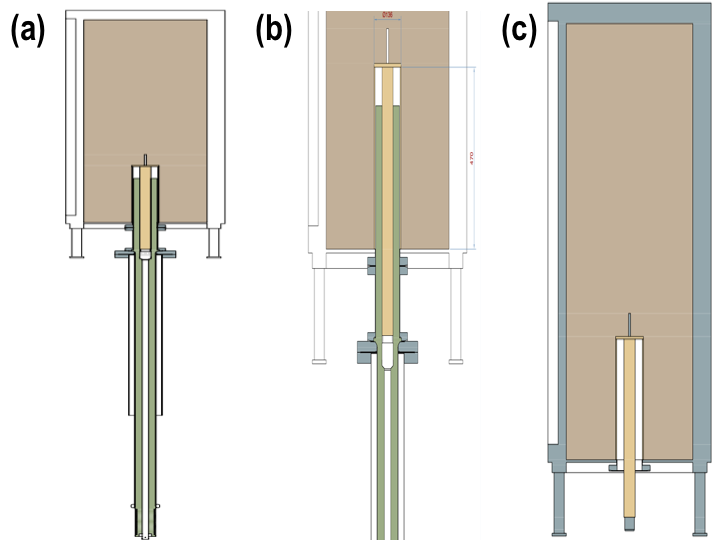
\includegraphics[width=0.5\textwidth]{DP_HVS_dp-hvps-750kv.png}
\end{dunefigure}


Typical Heinzinger power supplies have ripples in the range of $\sim$\SI{30}{k\hertz} with an amplitude of \SI{0.001}{\%V_{nom}} $\pm$ \SI{50}{mV}. A low-pass \dword{rc} filter designed to reduce the voltage ripple could be integrated into the output of the power supply.  It should be noted, however, that the required ripple suppression need not be as high as for the \dword{spmod} because the \dword{dpmod} has more effective shielding of the anodic structure, performed by the extraction grid and by the \dword{crp} signal amplification stage. 

%Assuming the distance between the power supply and the cathode to be \SI{15}{\m} and the capacitance of the \fdth and \dword{hv} extender to be about \SI{100}{\pF/\m}, a resistance of a few M$\Omega$ integrated at the output of the power supply is sufficient for noise reduction.

The \dword{hv} \fdth is based on the same successful ICARUS design adopted in both \dword{pdsp} and \dword{pddp}.  In this design, the voltage is transmitted along a stainless steel center conductor on the warm exterior of the cryostat, where this conductor mates with a cable end.  Inside the cryostat, the end of the center conductor has a spring-loaded tip that  contacts a receptacle cup mounted on the cathode, from which point \dword{hv} is delivered to the \dword{fc}.  The center conductor of the \fdth is surrounded by Ultra-High Molecular Weight Polyethylene (UHMW PE).  \fixme{Should this go into the common glossary?}


To first order, the upper bound of operating voltage on a \fdth is set by the maximum \efield on the \fdth.  Increasing the insulator radius reduces the \efield.  For the target voltage, the \fdth uses a UHMW PE cylinder of at least \SI{15.2}{\cm} (\SI{6}\,in) diameter.  In the gas space and into at least \SI{15.2}{\cm} of the liquid, a tight-fitting stainless steel ground tube surrounds the insulator.  The ground tube has a Conflat~\footnote{Conflat\texttrademark{}, \url{}.} 
\fixme{I can't find url for Conflat - anne}
flange of at least \SI{25.4}{\cm} (\SI{10}\,in) welded on for attachment to the cryostat.  A prototype\footnote{The prototype was manufactured by the company CINEL\texttrademark{} Strumenti Scientifici Srl.}  has been successfully tested up to \SI{-300}{\kV} in pure argon in a dedicated set up; two similar prototypes are being installed in \dword{pdsp} and \dword{pddp}.


%%%%%%%%%%%%%%%%%%%%%%%%%%%%%%%%%%%%%%%%%
\subsection{High Voltage Extender and Voltage Degrader}

Because the \dword{hv} musto be guided from the top of the cryostat to the cathode (\SI{12}{\m} below the \dword{lar} surface), an extension of the \dword{hv} \fdth is required, as shown in Figure~\ref{fig:dp-hvft-extender} a, b, and c. The extender contains an inner conductor at \dptargetdriftvoltneg surrounded by an insulator. The extension runs the entire height of the drift volume, so metallic rings (degrader rings) are installed on the periphery of the extension close to the field-shaping ring. Each degrader ring is electrically connected to the field shaping ring at the same height thus guaranteeing that the \efield in the \lar between the extender and the \dword{fc} remains at 0.


\begin{dunefigure}[\dual HVFT and extender]{fig:dp-hvft-extender}{Sketches of \dword{hv} \fdth and \dword{hv} extender-degrader: a) Overview of the \dword{hv} FT, \dword{hv} extender, and the degrader chain; b) details of the top portion of the \dword{hv} extender and its connections to the field shaping rings; c) details of the \dword{hv} extender and degrader connection to the bottom part of the \dword{fc}, including the connection to the cathode plane.}
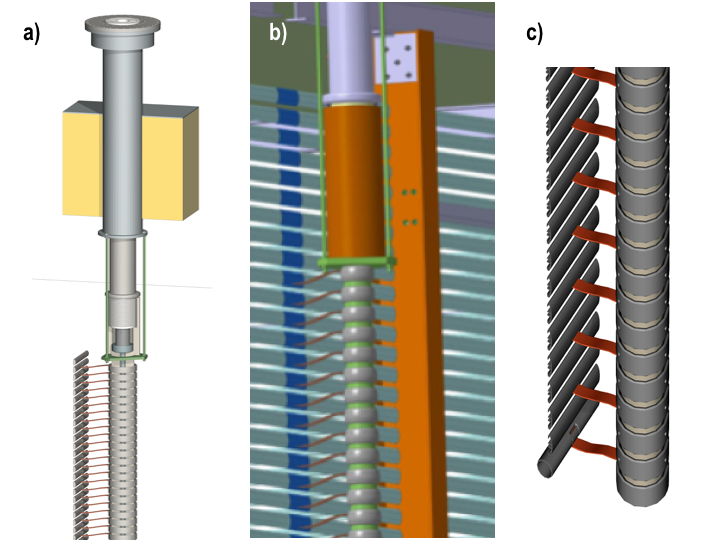
\includegraphics[width=0.75\textwidth]{DP_HVS_dp-hvft-extender.png}
\end{dunefigure}

%%%%%%%%%%%%%%%%%%%%%%%%%%%%
%\subsection{Cathode Plane and Ground Grid - 3 pages}

\subsection{Cathode Plane}

The \dpmod{}'s cathode plane forms the  bottom of the single 
\dptpcwdth (W) $\times$ \tpcheight (H) $\times$ \dptpclen
% \SI{12}{\m} (W) $\times$ \SI{12}{\m} (H) $\times$ \SI{60}{\m} (L) 
drift volume and provides a constant potential surface at \dptargetdriftvoltneg{}.  It receives its \dword{hv} from the central conductor of the extender that carries the voltage from the power supply through the \dword{hv} \fdth.  

The cathode plane consists of fifteen \SI{4}{\m} $\times$ \SI{12}{\m} modules. 
The cathode module design is based on the design used in  \dword{pddp}, with modifications to reach the \SI{12}{\m} span of the \dword{fd} and to implement features to electrically segment the cathode plane.

As shown in  Figure~\ref{fig:dune-dp-cathode}, each cathode module is constructed from two \SI{12}{\m} long trusses made from thin walled stainless steel tubes with approximately \SI{50}{\mm} outer diameter.  They can either be prefabricated and transported underground like the large cryostat beams, or assembled at the underground  cleanroom from shorter sections. The trusses are \SI{2}{\m} apart and are interconnected at both ends by two stainless steel tubes that serve as the outer edges of the cathode plane under the \dword{fc}. Resistive rods (\num{122} \SI{10}{\mm} diameter) are installed through the upper long tubes of the trusses at \SI{10}{\cm} pitch, forming the effective cathode plane. These rods are made from extruded FRP and wrapped with a layer of the resistive DuPont Kapton XC film also used on the \single \dword{cpa}s. These resistive rods have metal end caps to smooth out the sharp edges of the exposed resistive film and metal sleeves where they cross the trusses, so they can be locked down with screws. Preliminary mechanical analysis of the design shows that the deflection of the structure is approximately \SI{4}{\cm} when warm and about \num{60}~\% of that when in \dword{lar} (Figure~\ref{fig:dune-dp-cathode-deflection}).  The cathode modules are suspended to the matching FRP I-beams on the \dword{fc} modules along the two long walls of the cryostat. The resistive coupling between trusses/modules is achieved by custom resistive unions.  Each is made from a resistive sleeve, a G10/FR4 stiffening tube, and two locking rings. 


\begin{dunefigure}[A view of \dword{pddp} cathode module]{fig:dune-dp-cathode}
{A view of \dual cathode:  Construction uses a pair of stainless steel trusses as the framework with an array of FRP rods with resistive surfaces. The inset in the lower left shows the details of the resistive interconnect and the lifting tab on the cathode truss structure. The inset in the upper right is a detailed view of the components in a resistive union (Credit: BNL).}
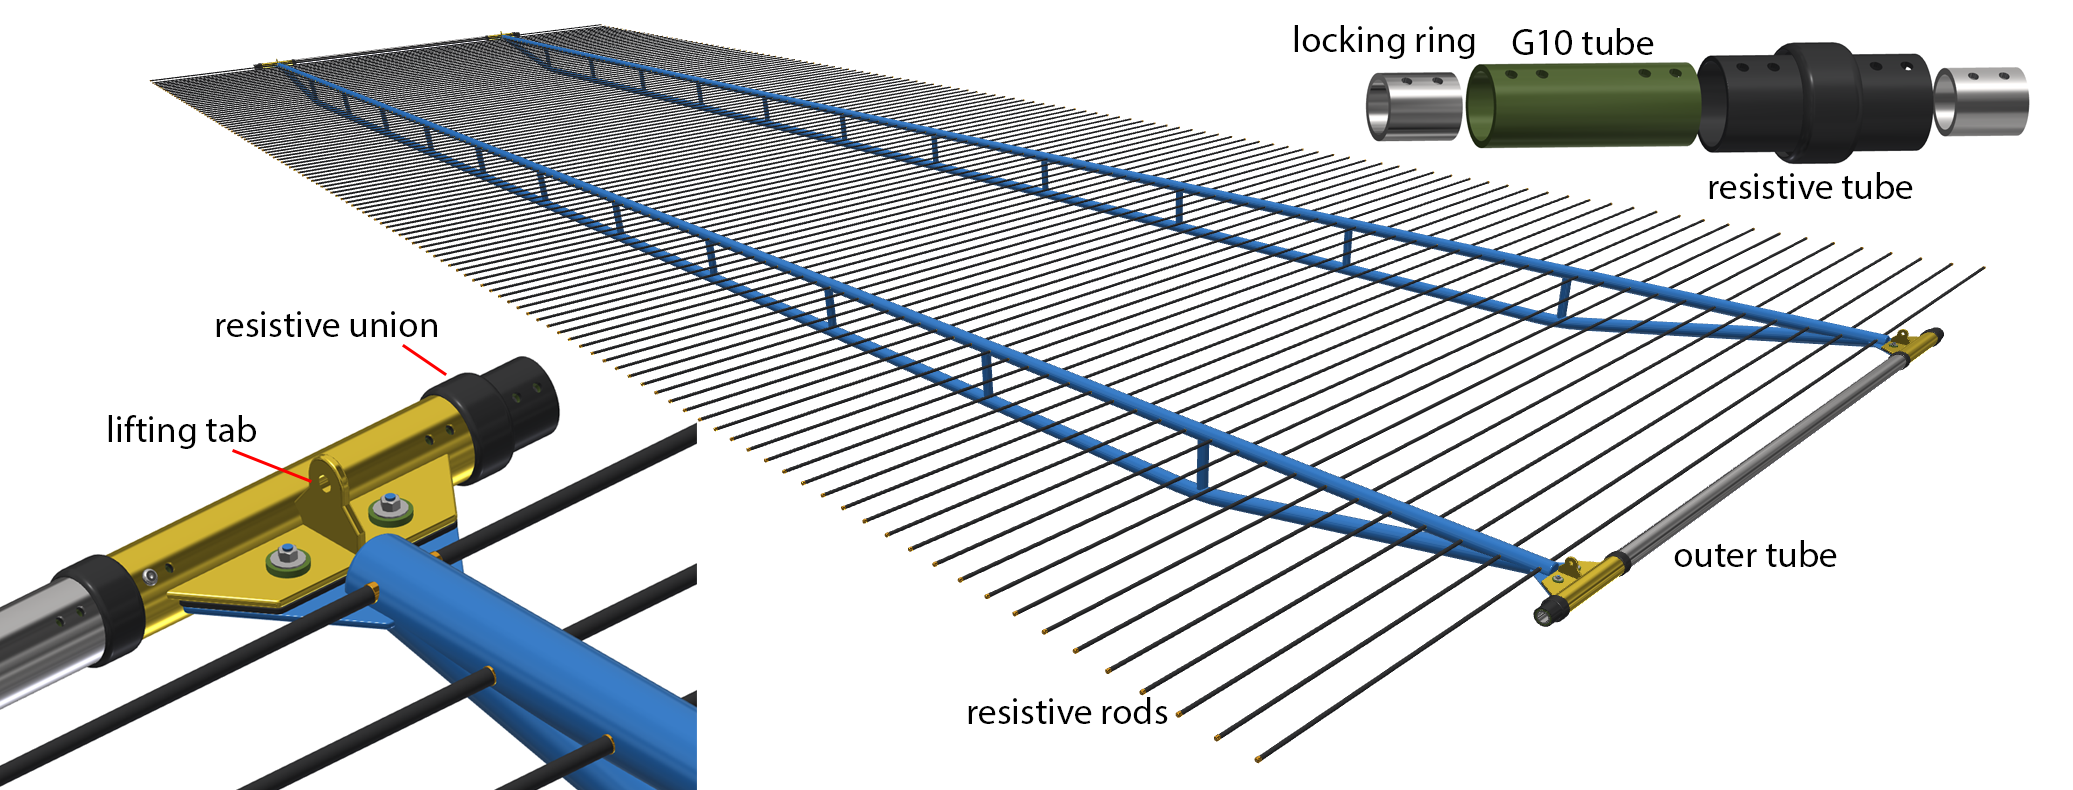
\includegraphics[width=0.9\textwidth]{DP_HVS_cathode_module.png}
\end{dunefigure}


\begin{dunefigure}[Deflection of the cathode truss]{fig:dune-dp-cathode-deflection}
{FEA of the cathode truss showing the deflection of the structure under its own weight and half of the weight of the FRP resistive rods at room temperature.  The deflection should reduce to approximately 60\% once the structure is submerged in liquid argon  (Credit: BNL).}
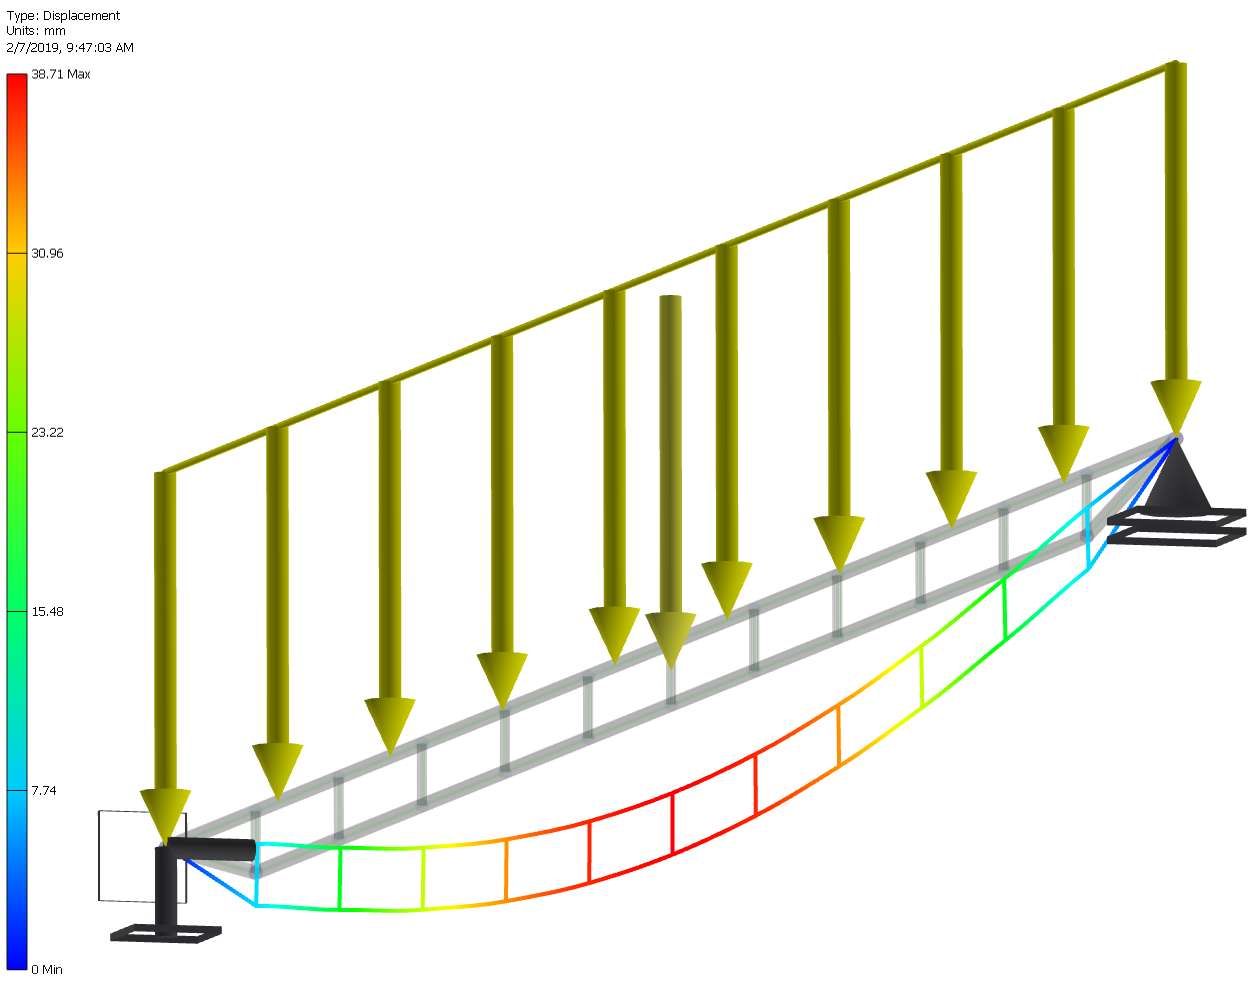
\includegraphics[width=0.7\textwidth]{DP_HVS_cathode_frame_FEA.png}
\end{dunefigure}


A \dword{hv} bus, made from \dword{hv} cable segments, is threaded through the outer tubes of all the cathode modules to form a conductive ring that distributes the cathode bias voltage.  The mounting plates (shown in gold in Figure~\ref{fig:dune-dp-cathode}) at both ends of a cathode truss are directly connected to the \dword{hv} bus through metal rings inside the tube.  These mounting plates are also connected to the \dword{fc} resistive divider chains. Between the mounting plate and the cyan colored truss, a layer of resistive sheet provides an additional barrier to energy transfer.  The resistivity of this sheet will be chosen to ensure the ionization current from $^{39}$Ar activities and the ion feedback from the LEM multiplication will not cause significant voltage drop on the cathode.


The energy stored in the volume between the cathode plane and the \dword{gg} (which sits under the cathode and above the \dwords{pd}) is estimated to be approximately \SI{1.7}{\kilo\joule} over the \dptpcwdth $\times$ \dptpclen area, based on the cathode voltage and the distance of \SI{1}{\m} between the cathode and the \dword{gg} described in Section~\ref{sec:dp-hv-groundgrid}. 
A sudden discharge from the cathode frame to the cryostat membrane could cause severe damage to both.
  The modular construction of the cathode helps minimize this effect in case of discharge. During assembly in the cryostat, the cathode units are kept electrically insulated and connected to their immediately adjacent neighbors through \si{\giga\ohm}  
resistors. Given the \SI{100}{\pico\farad} capacitance of each cathode unit, any discharge occurring in one unit will release at most 
\SI{21}{\joule} of stored energy while the discharge rate  
to the other units is slowed to the several-hundred-millisecond range.

Detailed calculations are in progress to determine the final shape and the size of the cathode and \dword{gg} frames to %meet the requirement that 
limit the maximum \efield to \SI{30}{\kV\per\cm}  
throughout the \lar volume (Figure~\ref{fig:dune-dp-cathode-field}) (see Requirement 2 in Table~\ref{tab:hvphysicsreqs}).  Structural calculations must also verify the planarity of the cathode as it hangs on the \dword{fc} supports.
Values and voltage characteristics of the connecting resistors will also be defined according to results from dedicated simulations of the cathode electrical model.


\subsection{Ground Grid}~\label{sec:dp-hv-groundgrid}

An array of ground grid modules is installed between the \dwords{pmt} and the cathode plane to provide a low E field environment for the \dwords{pmt} and shield them from an \dword{hv} discharge from the cathode plane.

The ground grid modules are made from 304 stainless steel tubes.  Each covers \num{3} $\times$ \num{3} \dword{pmt} modules at \SI{1.02}{\m} pitch. The modules are placed on the cryostat floor at a pitch of \SI{3.06}{\m}. The \num{4} legs are \SI{2.72}{\m} apart, aligned with \SI{0.34}{\m} pitch of the membrane corrugation so that the feet are always on the flat part of the membrane. The modules are not physically in contact with each other, which means they can be individually read out to monitor \dword{hv} stability. To avoid damage to the membrane floor, the feet will be covered with a Teflon \fixme{Should this have the copyright mark?} sheet.  Electrical contact to the membrane (detector ground) will be made with springs through the Teflon sheet, and grounding wires to the edges of the cryostat. To cover the entire cathode, a total of \num{80} ground grid modules in the form of a \num{4} $\times$ \num{20} array will be needed. Preliminary analysis on the ground grid structure shows we can expect approximately \SI{1}{\cm} sagging in the center of grid. Detailed studies of the grid geometry are ongoing to ensure that the requirement for the maximum local field is satisfied. Figure~\ref{fig:dune-dp-cathode-field} shows the surface E field on the cathode and ground grid near a cathode edge.  The maximum E field is under the curved section of the lower truss member at the 30kV/cm \fixme{This should use LATEX coding.} limit.

\begin{dunefigure}[A single ground grid module]{fig:dp_hvs_ground_grid}
{Left: A view of a ground grid module; Right: ground grid position relative to the membrane corrugation and \dword{pmt} locations (Credit BNL).}
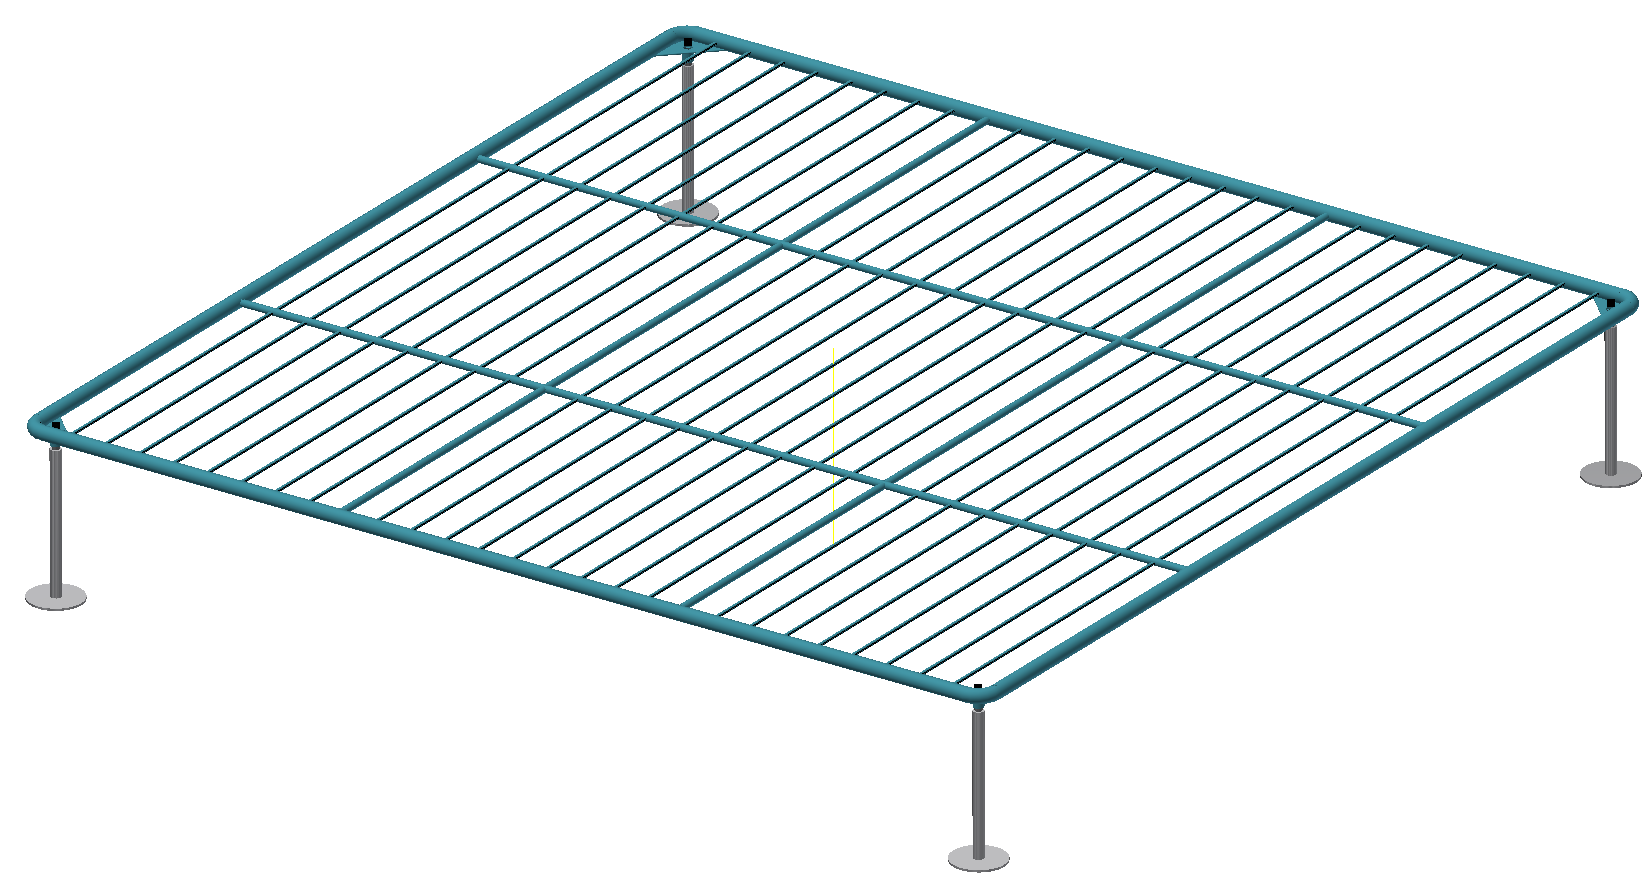
\includegraphics[width=0.6\textwidth]{DP_HVS_ground_grid_3x3.png}
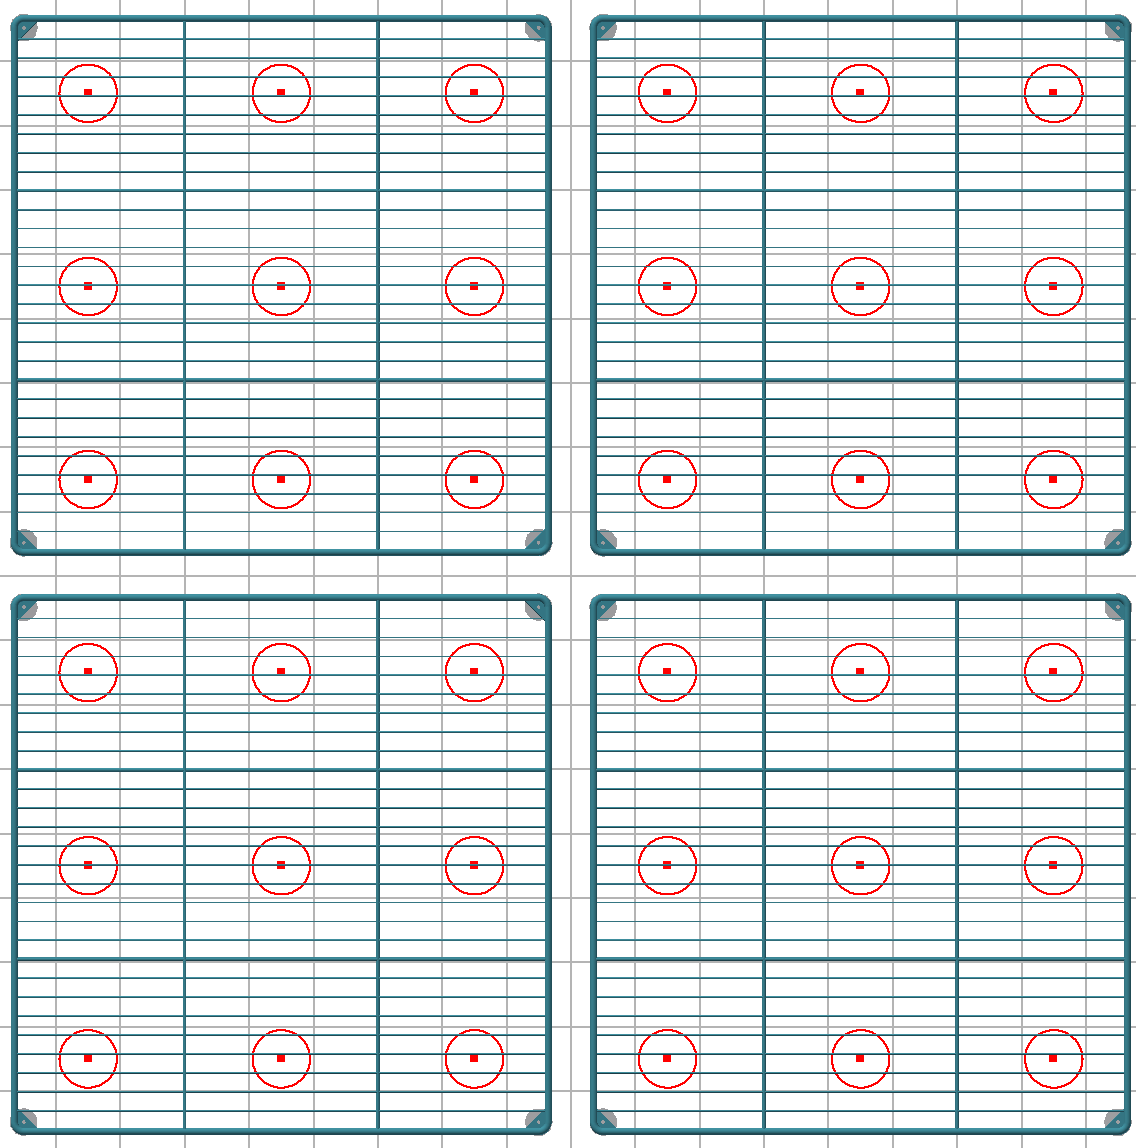
\includegraphics[width=0.3\textwidth]{DP_HVS_ground_grid_plan_view.png}
\end{dunefigure}


\begin{dunefigure}[\dword{pddp} cathode field]{fig:dune-dp-cathode-field}
{Electrostatic calculation of the surface electric field on a section of the cathode (upper) and ground grid (lower) structures. The outer tube and the bottom tube of the cathode structure have high surface electric field.   The maximum E field is approximately 30kV/cm \fixme{This should be in LATEX code.} at the curved section of the bottom tube (Credit: BNL).} 
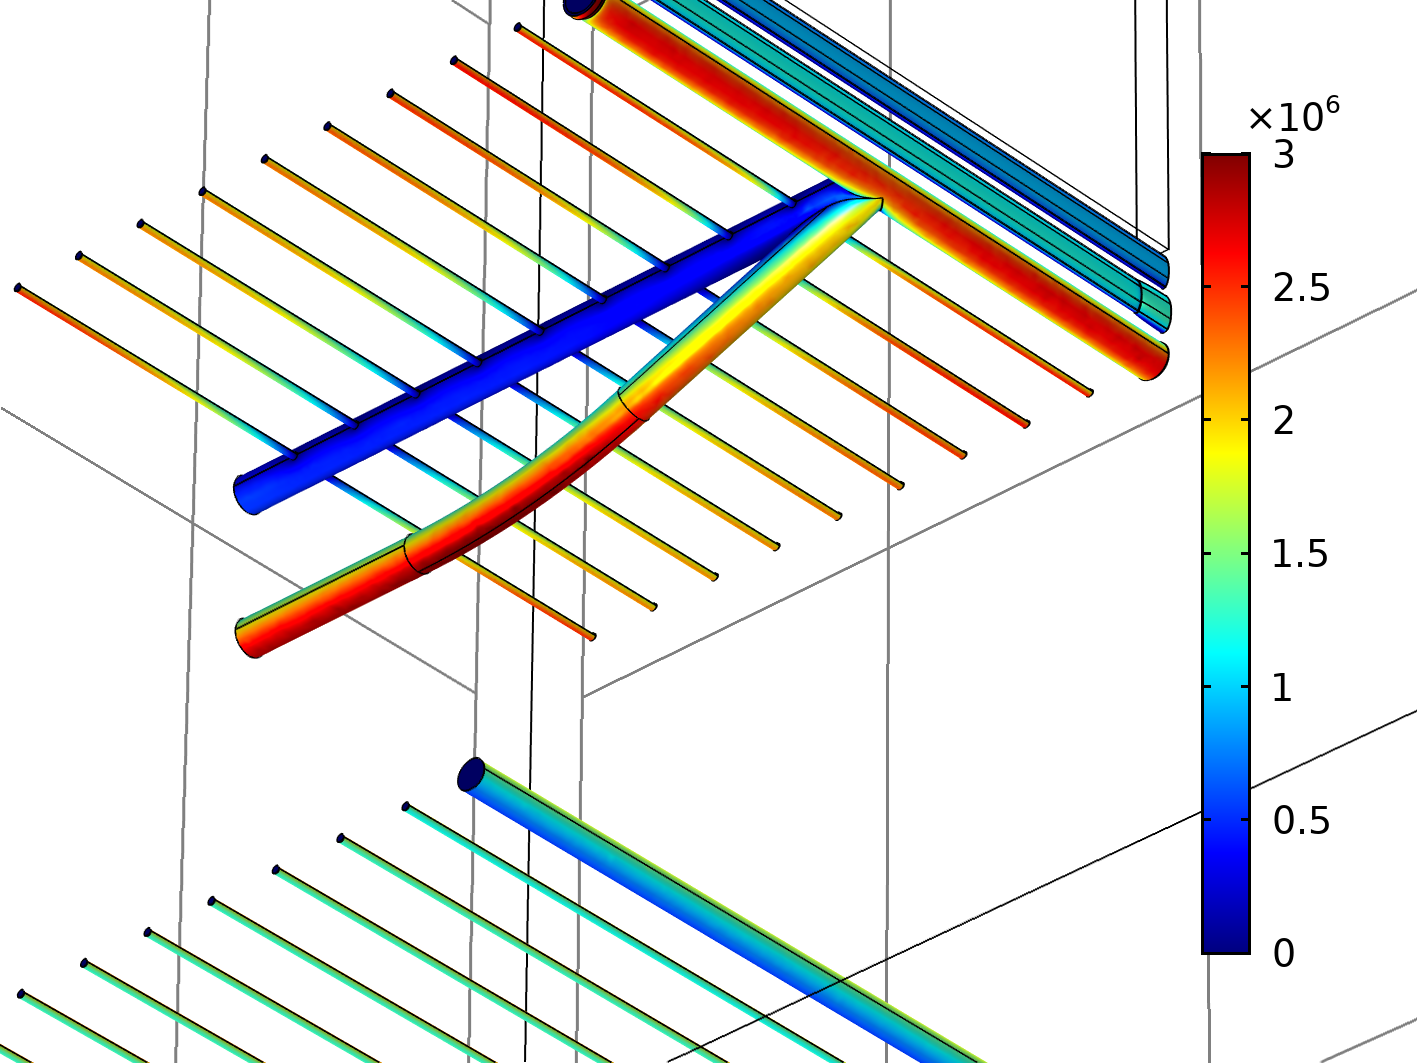
\includegraphics[width=0.7\textwidth]{DP_HVS_cathode_E_field2.png}
\end{dunefigure}


\subsection{Field Cage - 4 pages}

The field shaping rings of the \dword{fc} are made of extruded aluminum open profiles.  
The profiles are interconnected horizontally through resistive joints into closed rectangular loops. The four walls surrounding the \dword{tpc}'s active volume are formed using \num{199} of these loops stacked vertically. The aluminum profiles are attached to structural elements made of pultruded Fiber Reinforced Plastic (FRP). \fixme{This abbreviation is used frequently in this chapter, but it is not in the common glossary. It probably should be.}

FRP is non-conductive and strong enough to withstand the \dword{fc} loads. %in the temperature range of \SI{-150}{\degreeCelsius} to \SI{23}{\degreeCelsius}.
This material meets the  Class A International Building Code classification for flame spread and smoke development, 
as characterized by ASTM E84. 

The entire \dword{fc} is constructed from \num{12} super-modules with nominal dimensions of \SI{12}{\m} width and \SI{12}{\m} height. There are \num{5} super-modules each along each long wall, and one each along the \endwall{}s.  The inner surfaces of the \dword{fc} profiles are positioned \SI{15}{\cm} away from the \dword{crp}'s active area to allow the \dword{fc} support structure to pass through and to provide a uniform drift field.  For the tilted \endwall super-modules, this \SI{15}{\cm} offset applies only to their top edges. Each super-module, including their top steel beam, weighs about \SI{1200}{\kg}.

Each super-module is built from an array of \num{3} wide by \num{6} high sub-modules. All sub-modules share the same basic construction: two \SI{10}{\cm} (H) $\times$ \SI{5}{\cm} (W) FRP I-beams with two stainless steel cross bars that form a rigid frame structure. Profiles, \num{33} or \num{34} (bottom row sub-module) and \SI{4}{\m} long, are mounted at \SI{6}{\cm} pitch on one side of the frame structure using screws and slip nuts inside the profiles. Most of the sub-modules are \SI{4}{\m} (W) $\times$ \SI{1.98}{\m} (H). Figure~\ref{fig:dune-dp-fc-module} shows the design of a non-corner \dword{fc} sub-module. 


The extruded aluminum profiles are mounted on one surface of the flange of the \SI{10.2}{\cm} (\SI{4}{in}) FRP I-beam via two stainless screws and aluminum slip nuts in the center enforcement rail of the profile. The mounting is fully secured only on one of the \SI{10.2}{\cm} I-beams flange and loosely on the other but sufficiently secured to hold the profile in place. This prevents the contraction on either side of the profile from straining the profile. The top sub-module has an extended \SI{10.2}{\cm} FRP beam with holes to connect it to the stainless steel I-beam hanging from the ceiling. The bottom sub-module has a cutout to hold the cathode plane onto it. The four middle sub-modules are symmetric and thus interchangeable.


The corner sub-modules have similar construction, but with features specific to their locations. On an \endwall super-module, the corner modules have \num{90} degree bent profiles one one side. Along the long walls, the modules near the \endwall{}s have profiles cut at different lengths to accommodate the \num{2.4} degree incline of the \endwall super-modules.

The \endwall \dword{fc} modules also have a slightly larger pitch between the \dword{fc} profiles to ensure proper alignment when tilted at the designed angle.  The profiles are also mounted with a slight angle against the FRP I-beams by means of slightly tapered spacers.

Approximately \SI{500}{\N} of force is needed to keep the \endwall \dword{fc} super-modules inclined. This force is transferred through the interconnected cathode outer tubes to keep the opposite \endwall super-module inclined in a symmetrical pattern. There will be a few centimeters of sag in the middle of the \endwall, which will not affect the \dword{tpc} operation.   

%The \dword{fc} is modular, each module covering a vertical area of \SI{4}{\m} (W) $\times$ \tpcheight (H). 
%There are two types of modules, straight section and corner, both types having the dimensions \SI{4}{\m} (W) $\times$ \tpcheight (H). A total of \num{76} straight section modules (i.e., with straight profiles) and four corner section modules, with profiles bent \num{90} degrees at one corner to allow straight connections via resistive sheaths around the corner on the straight section on the SWSM, as shown in Figure~\ref{fig:dune-dp-fc-all}.c.  A photo of the \dword{pddp} \dword{fc} is shown in Figure~\ref{fig:dune-dp-fc-all}.d.

\begin{dunefigure}[ \dword{fc} module view]{fig:dune-dp-fc-module}
{Sketches of an \dword{fc} sub-module viewed from inside the field cage (bottom) and outside the field cage (top), along with a photo of a partly completed sub-module and a close up cross section of a profile attached to the FRP using a slipnut.  The inside view shows the two vertical FRP I-beams and two horizontal metal cross bars forming the structural frame work on which \num{33} \SI{4}{\m} long aluminum profiles are attached.  A series of resistive divider boards interconnect all the profiles to provide a linear voltage distribution. The outside view shows that outer surface of the \dword{fc} module is insulator free to avoid \dword{hv} instabilities due to surface charging (Credit: BNL).
}
%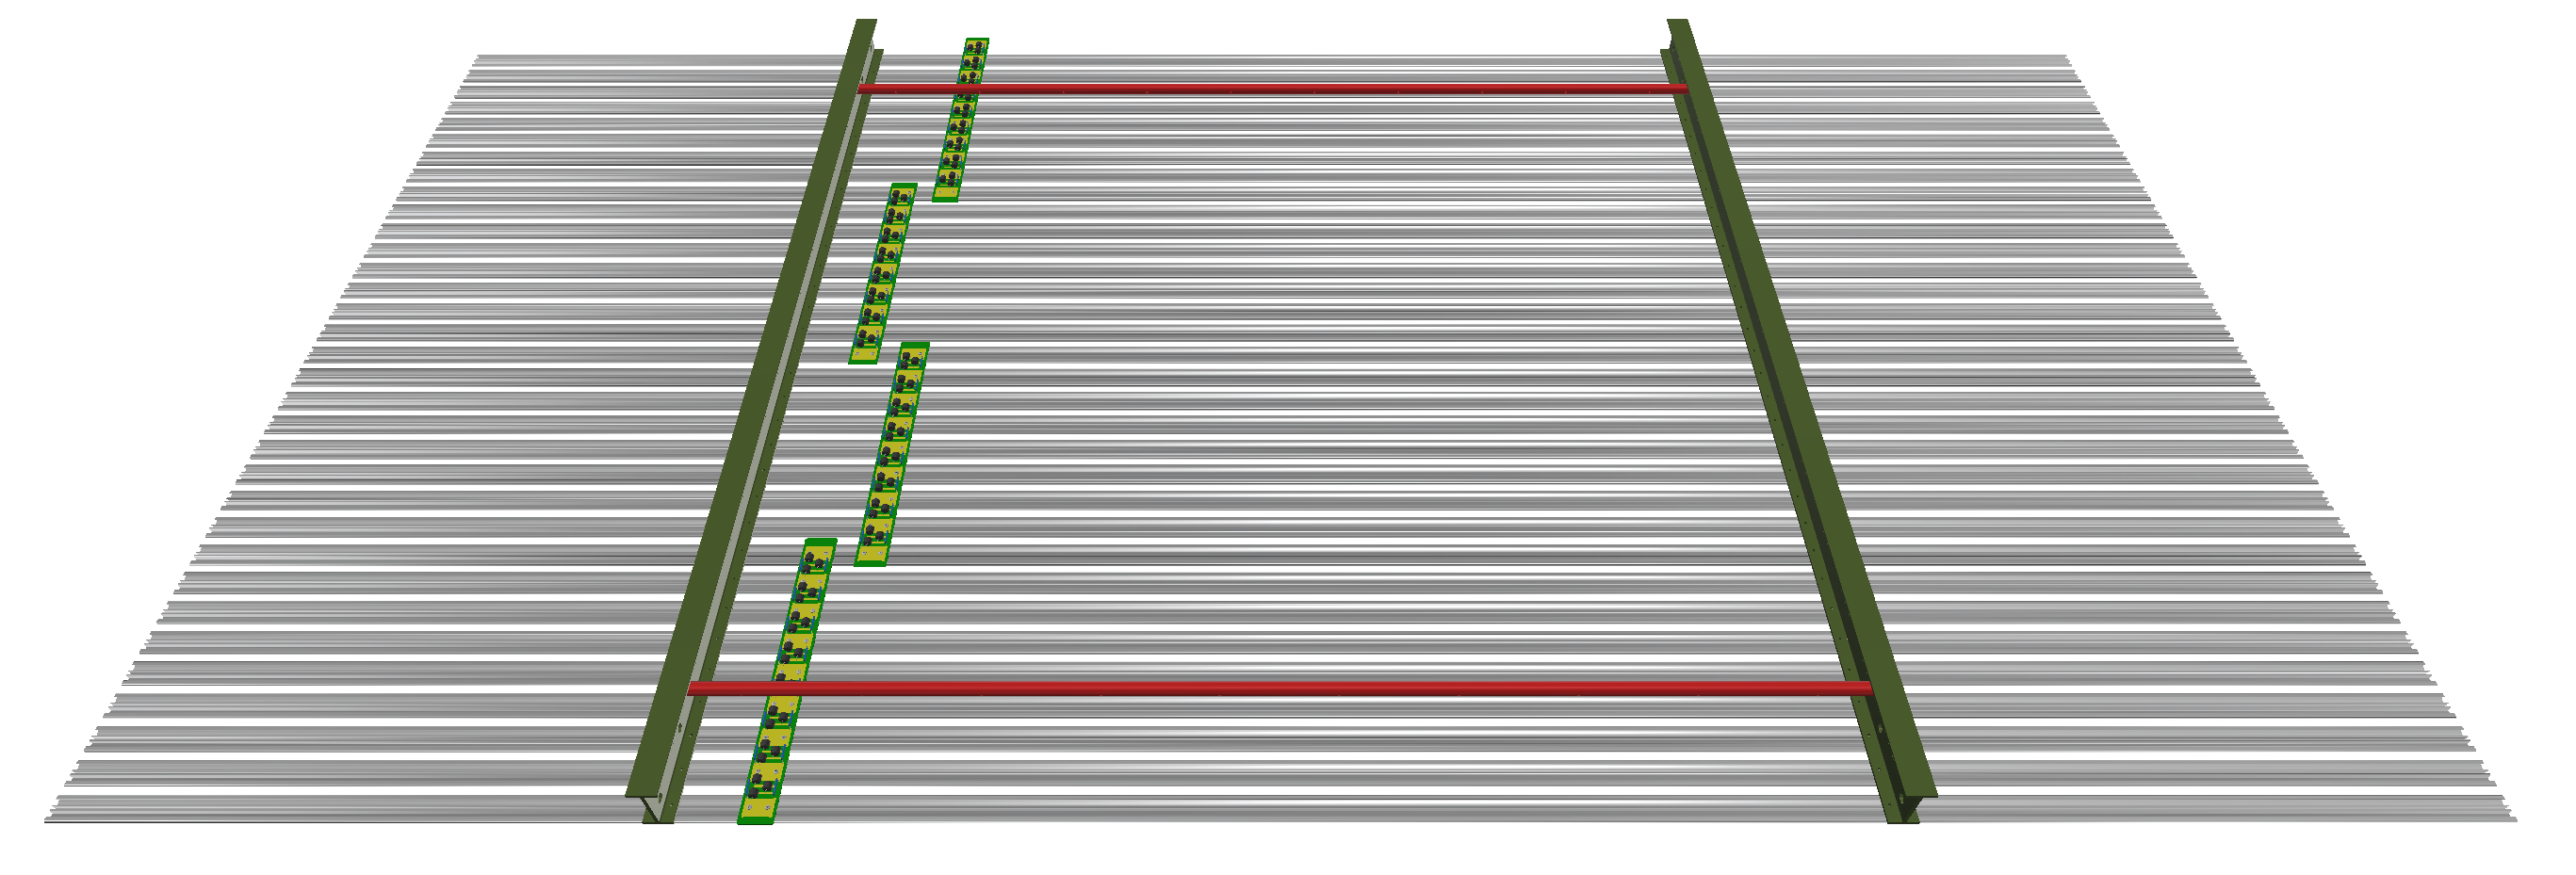
\includegraphics[width=0.9\textwidth]{graphics/DP_HVS_FC_Bottom_Module_Middle.png}
%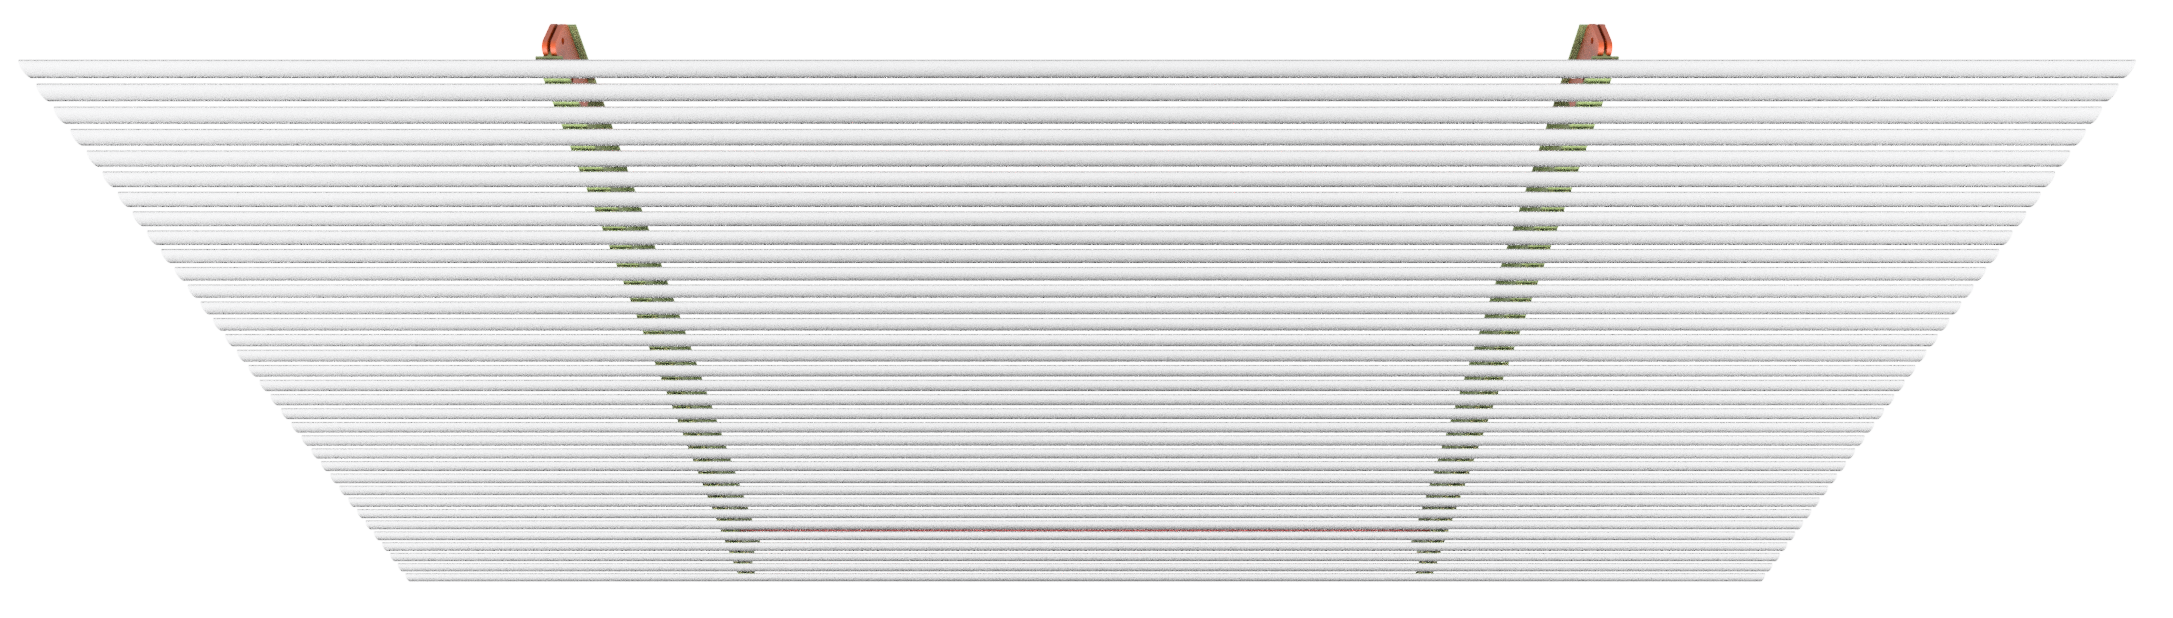
\includegraphics[width=0.9\textwidth]{graphics/DP_HVS__FC_Super_Module_Middle_Outside.png}
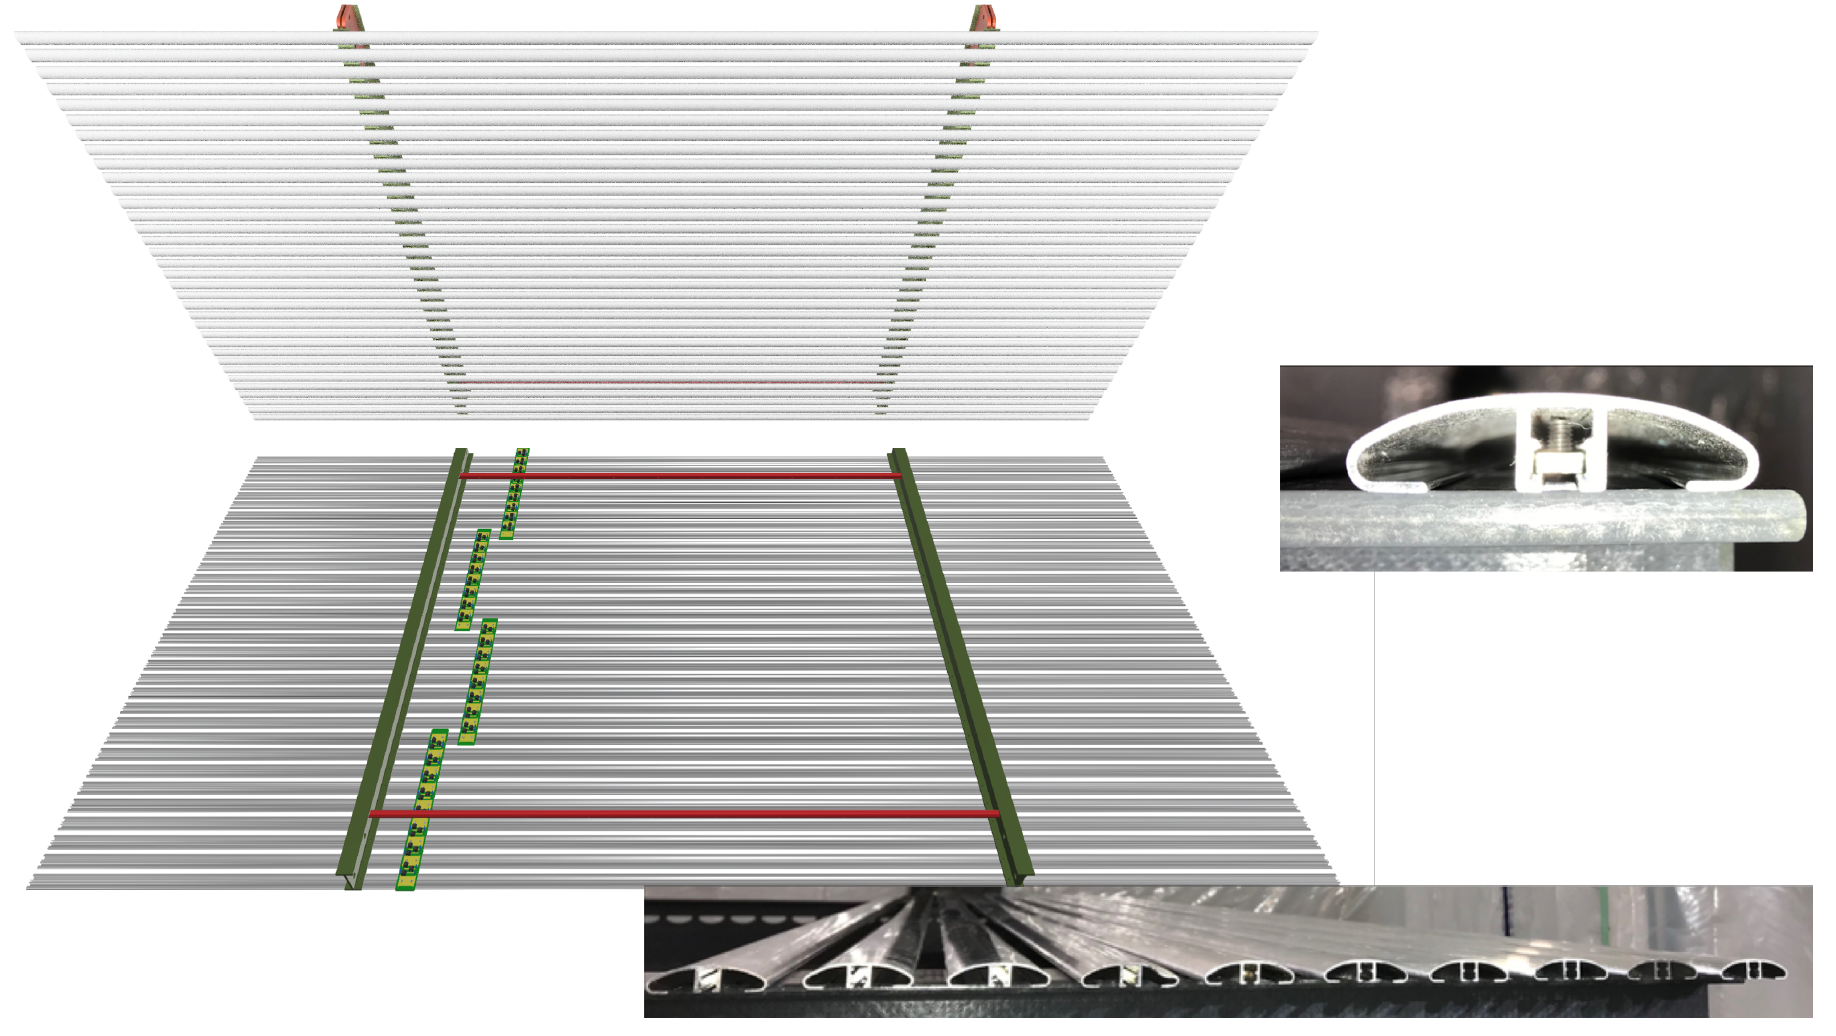
\includegraphics[width=0.9\textwidth]{DP_HVS_FC_Sub_Module.png}
\end{dunefigure}

\begin{dunefigure}[ \dword{fc}-cathode corner]{fig:dune-dp-fc-cathode-corner}
{A view of a bottom corner of the field cage showing the \num{90} degree bent \dword{fc} profiles on the \endwall module and the cathode structure near the \endwall (Credit BNL).}
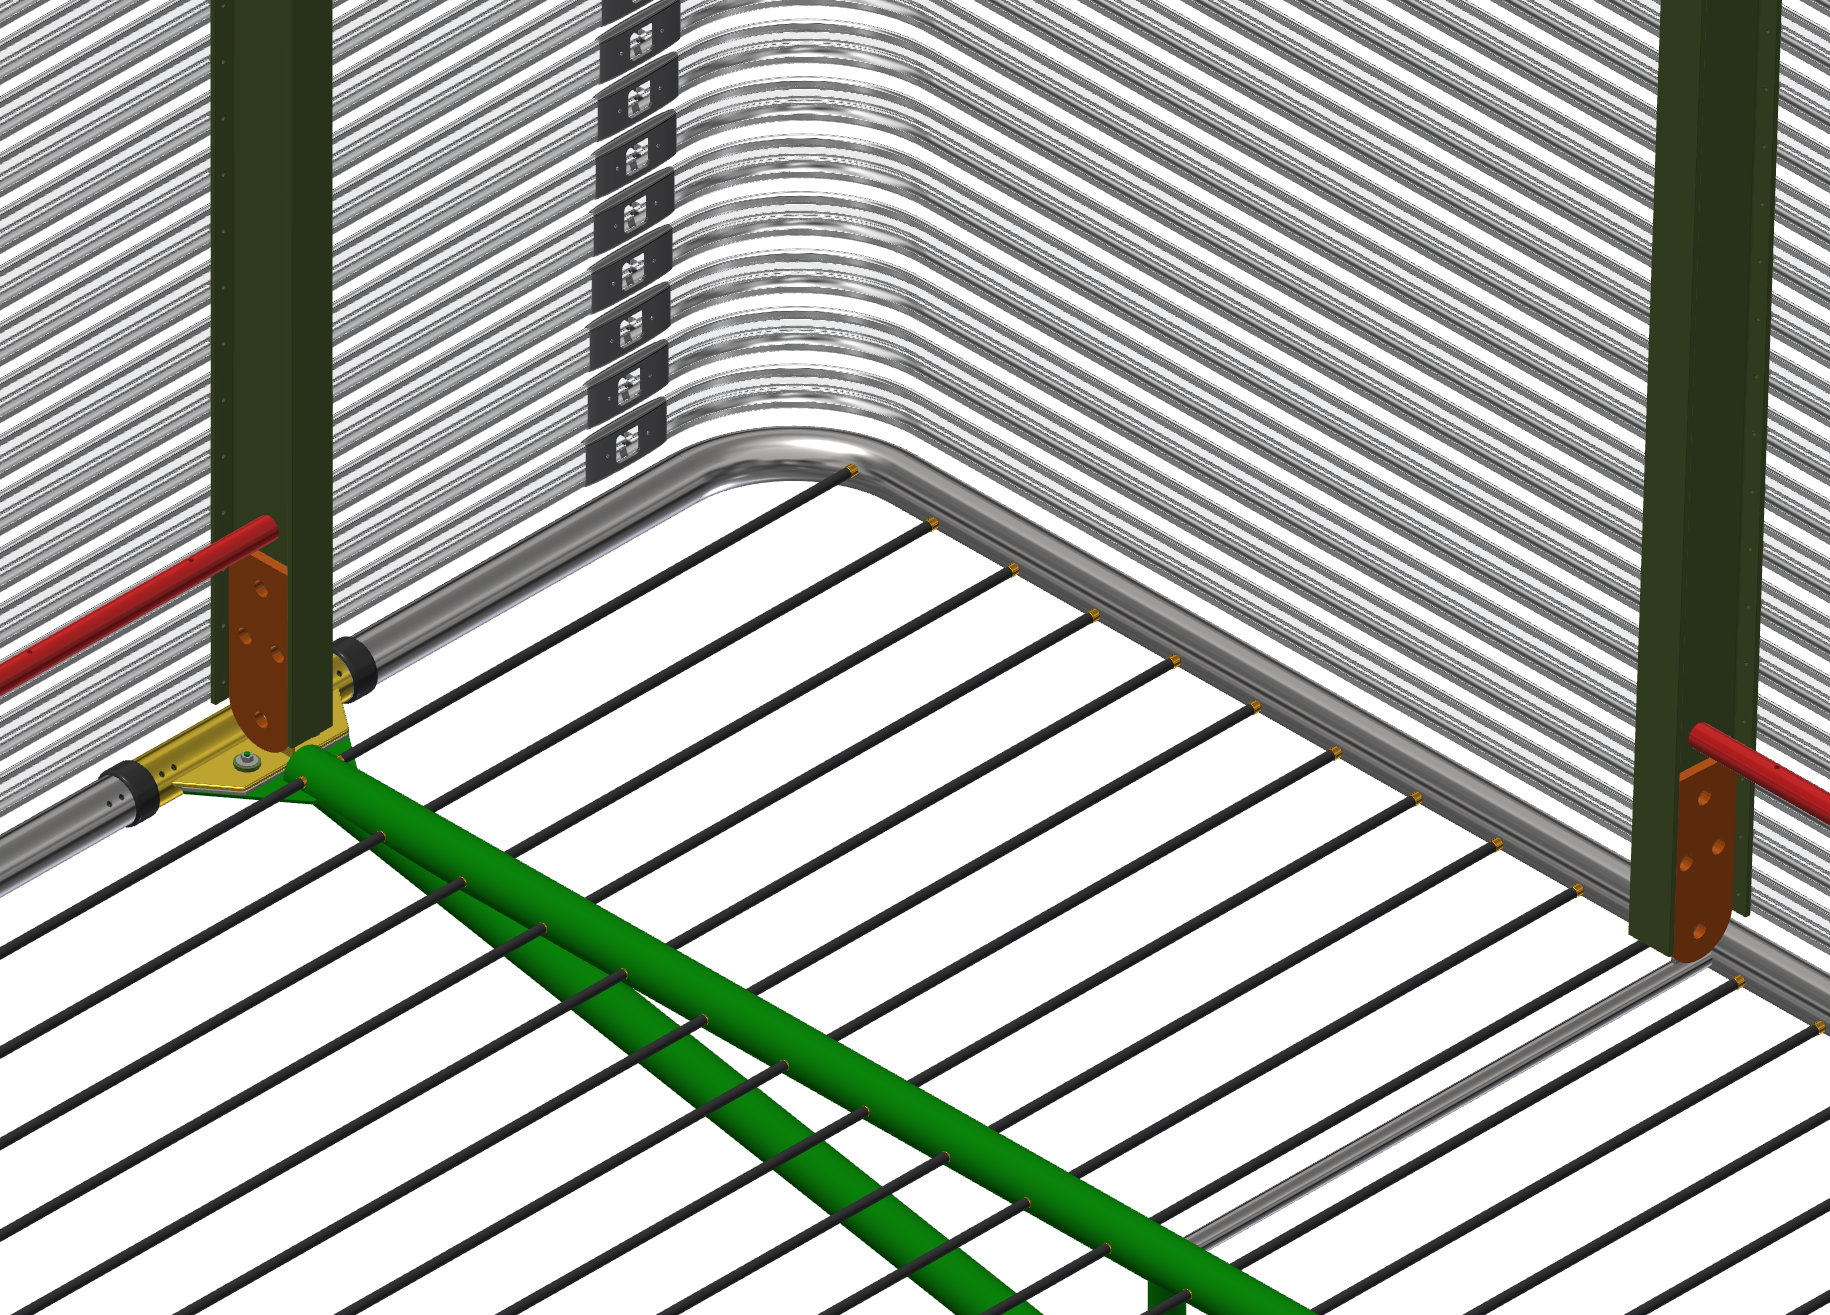
\includegraphics[width=0.9\textwidth]{DP_HVS_EW_corner_details.png}
\end{dunefigure}

\begin{dunefigure}[ \dword{fc} elevation]{fig:dune-dp-fc-elevation}
{A side view of one end of the \dword{hv} system components in the \dword{tpc} showing the top frame, left-most super-module with profiles, and the ground grid array on the bottom.  The \endwall super-module on the left is pushed away from the cryostat wall by \SI{0.5}{\m} on the bottom to gain additional \dword{hv} clearance (Credit: BNL).}
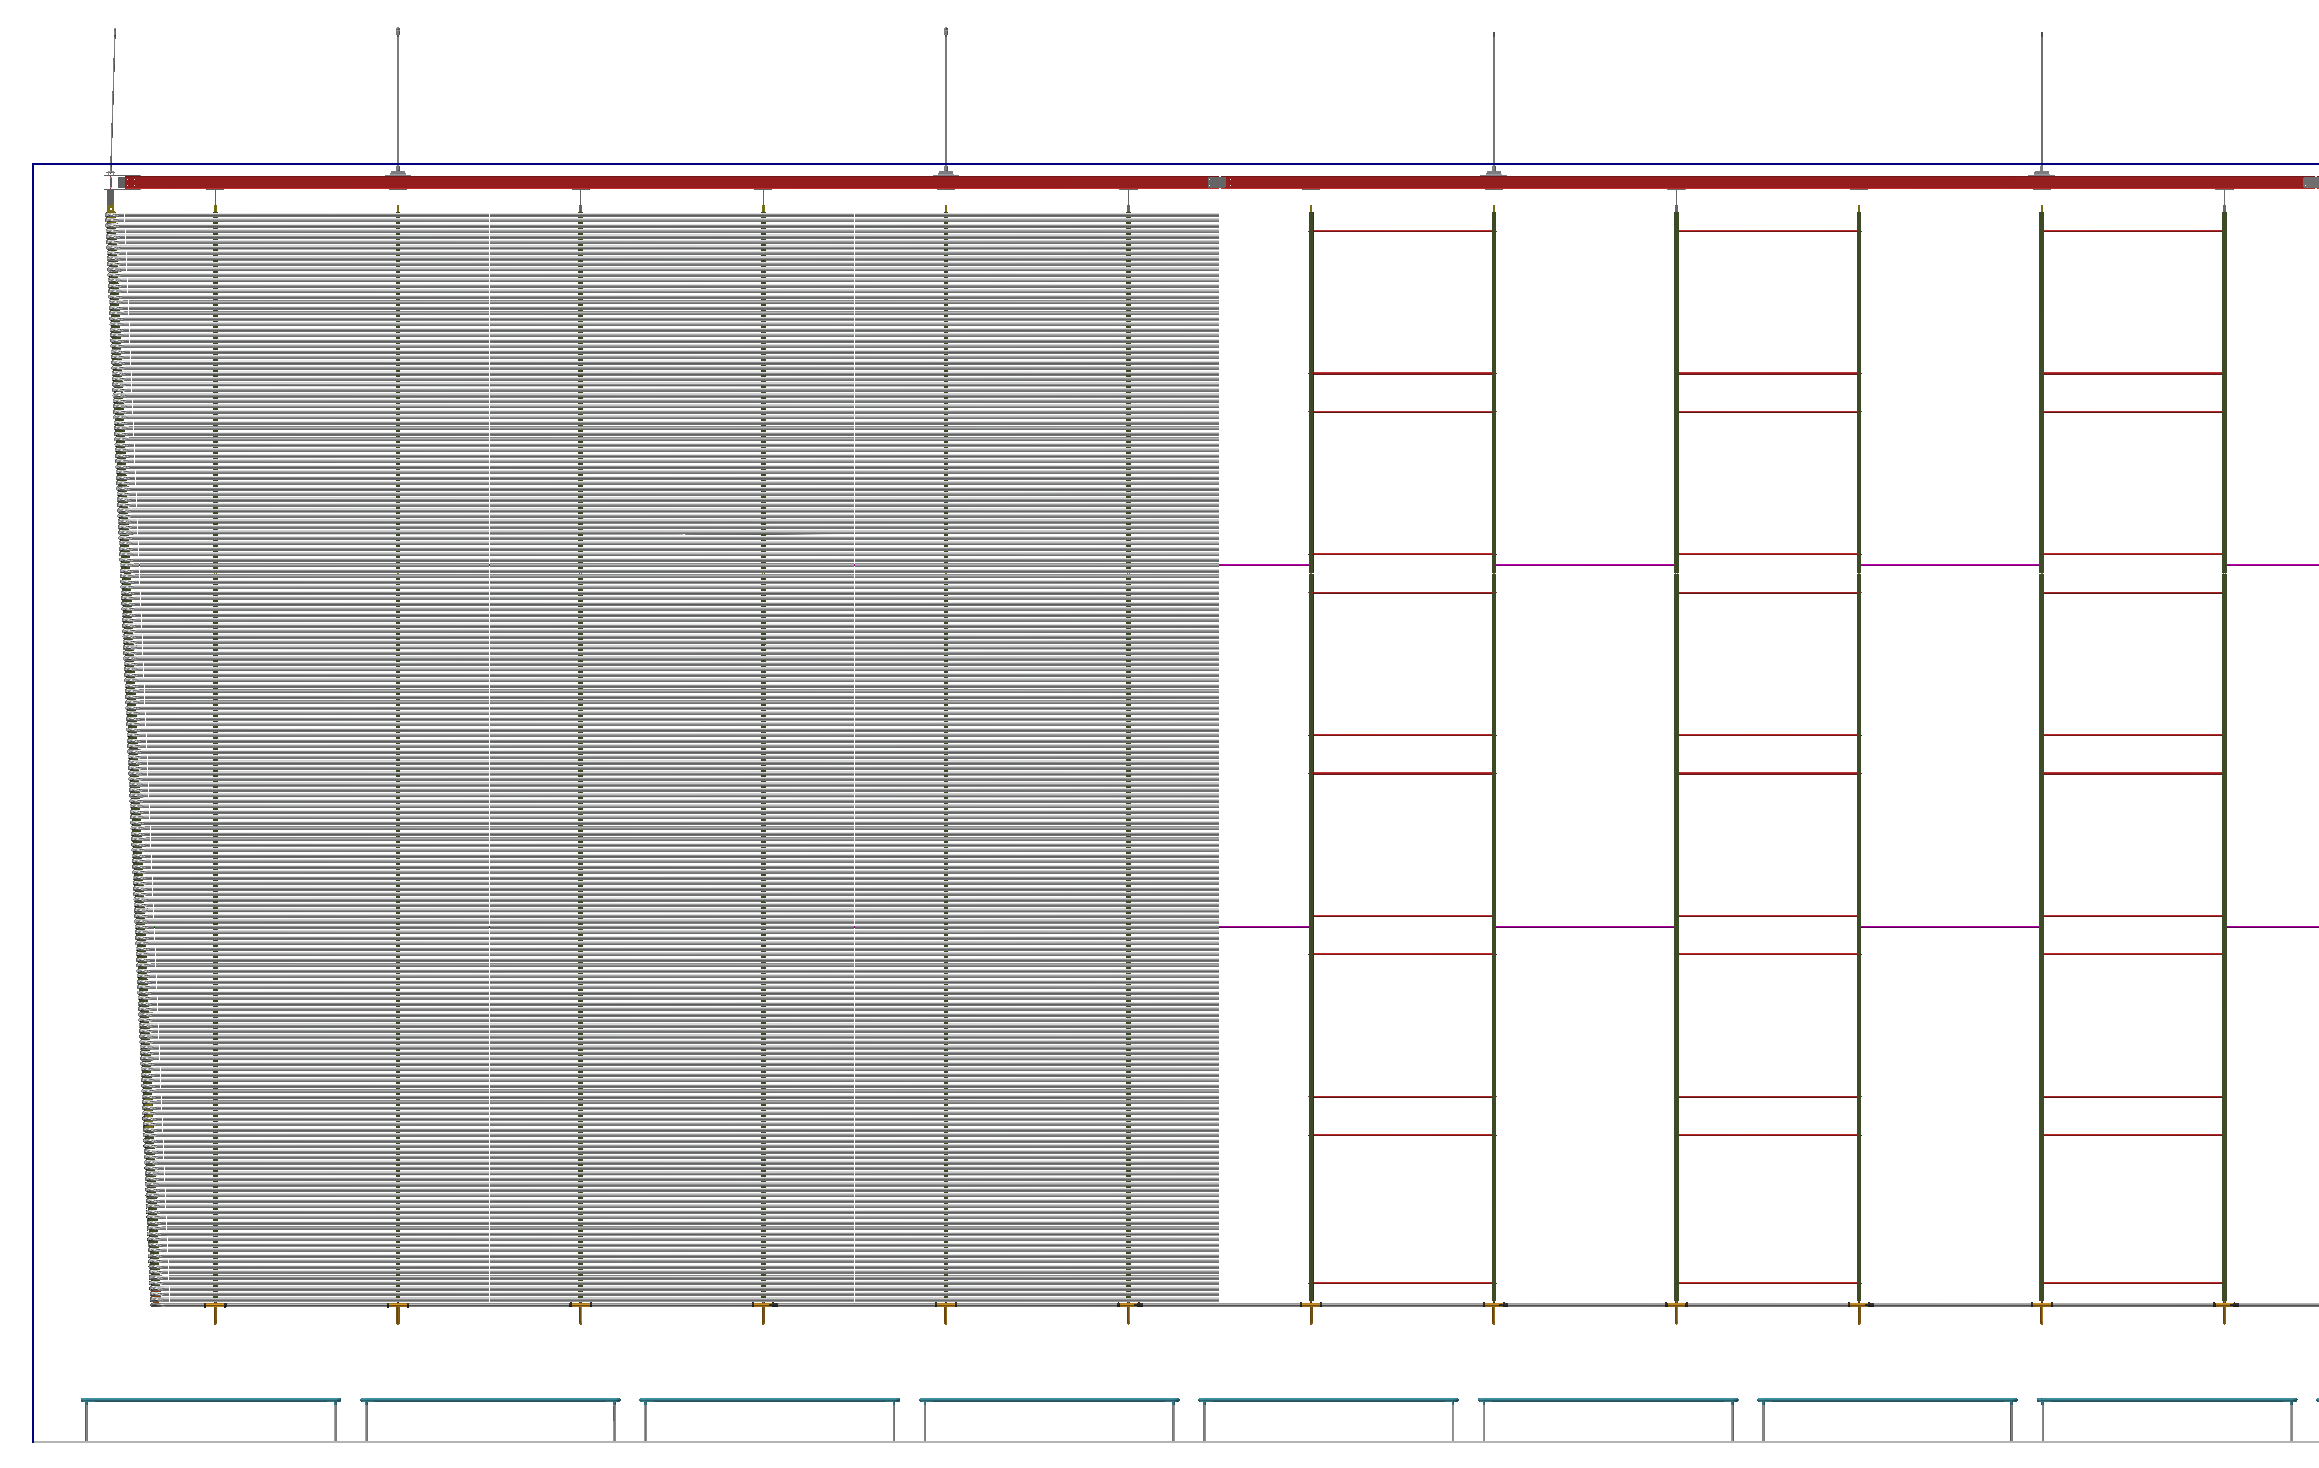
\includegraphics[width=0.95\textwidth]{DP_HVS_FC_elevation.png}
\end{dunefigure}


\begin{dunefigure}[\dword{fc} interconnections]{fig:dune-dp-fc-interconnection}
{Left: Interconnect details between \dword{fc} sub-modules; Right: Interconnect details between the bottom \dword{fc} sub-module and the cathode structure. All metal fasteners used here are aligned with the centers of nearby \dword{fc} profiles and connected electrically to the \dword{fc} profiles at the same height (Credit: BNL). }
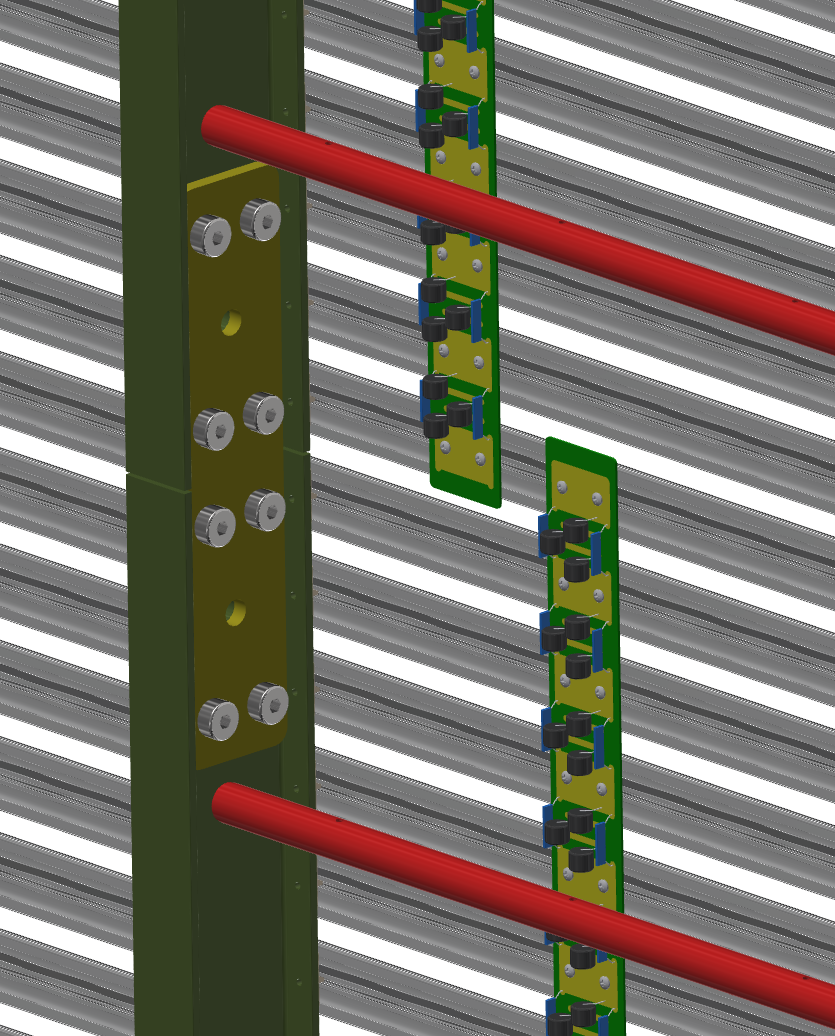
\includegraphics[width=.45\textwidth]{DP_HVS_FC_module_interconnect_details.png}
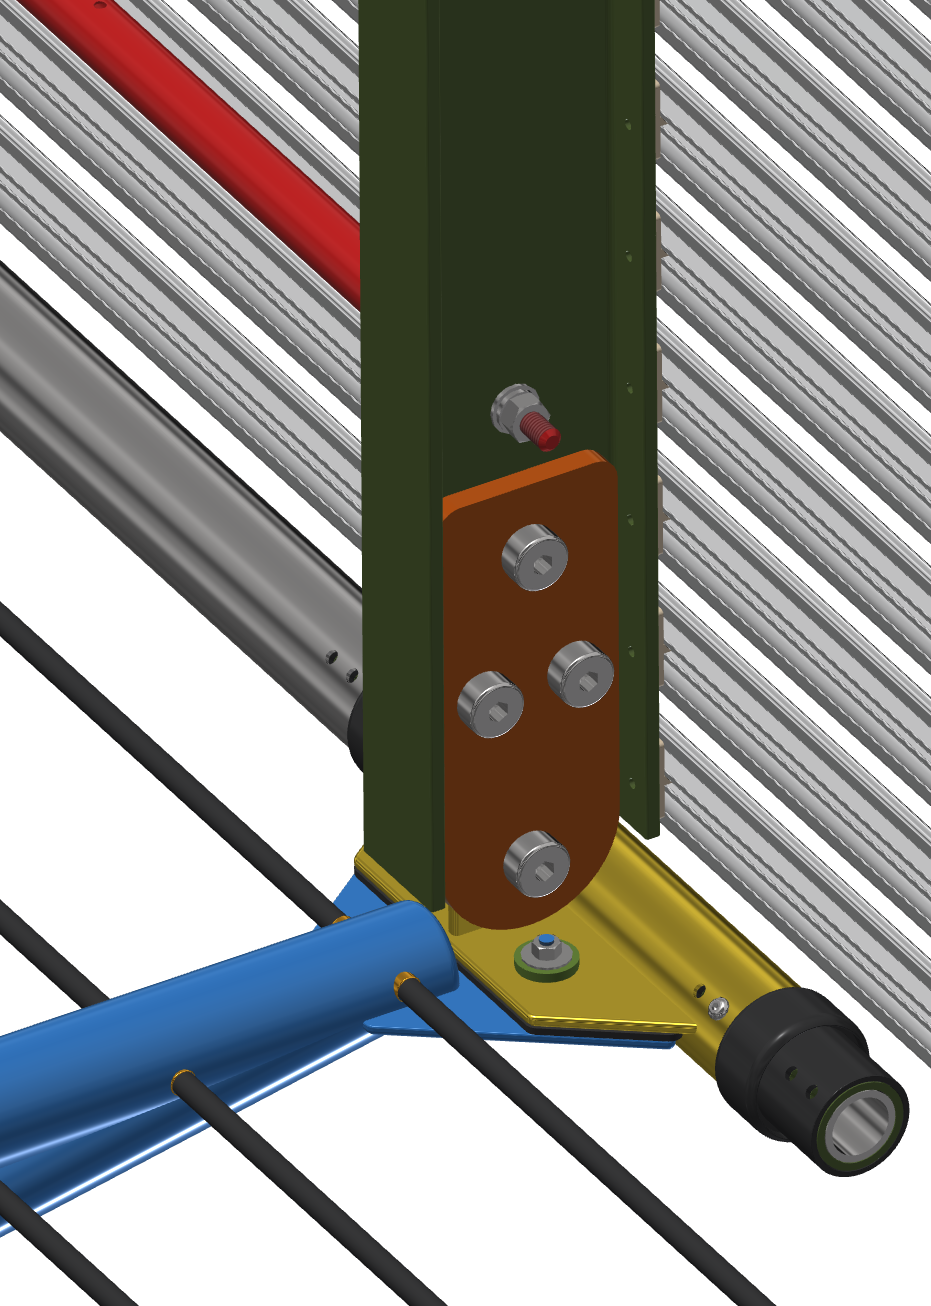
\includegraphics[width=.4\textwidth]{DP_HVS_FC_cathode_connection_details.png}
\end{dunefigure}

Each full height \dword{fc} module is made of six sub-modules of three distinct types: top, bottom, and middle. The dimensions for all sub-modules are \SI{4}{\m} (W) $\times$ \SI{2}{\m} (H).
Each module has one top sub-module with \num{33} profiles, four middle sub-modules with \num{33} profiles each, and one bottom sub-module with \num{34} profiles, for a total of \num{199} profiles per module. 
The voltage of the top-most field shaping ring is \SI{-9}{\kV}. 
The top sub-module makes the mechanical connection to the ceiling of the cryostat from which the entire \dword{fc} hangs, as shown in Figure~\ref{fig:dp-fc-installation-connection}, left. The bottom modules make both mechanical and electrical connections to the cathode. 

\subsection{Electrical Interconnections}
A railed rib runs along the length of the aluminum profiles at the center of the profile.  The rib provides mechanical strength and acts as a rail for the slip nuts that hold the profiles onto the supporting FRP frame. The rib also serves as a rail for the square nuts that hold the \dword{hv} divider boards both mechanically and electrically and the nuts for securing the resistive sheath whose CAD drawings are shown in Figure~\ref{fig:resistive-sheath} a and b. 

All profiles at a given height are electrically connected via a resistive sheath screwed onto a nut in the center enforcement rail across two neighboring profiles as depicted in Figure~\ref{fig:resistive-sheath} c and d with a 3D printed mock up plastic sheath with a profile inserted and screwed onto the sheath with a metal screw for a secure electrical connection. A resistive divider board chain interconnects the aluminum profiles to provide a linear voltage gradient between the cathode and the top field-shaping ring.   

\begin{dunefigure}[\dual \dword{fc} Resistive Sheath]{fig:resistive-sheath}
{a: Top view of a CAD drawing for the resistive sheath; b: Bottom view of the same CAD drawing; c: A cross-sectional photograph of the mock up plastic sheath screwed onto the profile center rib; d: The bottom view, active volume side, of a sheath connecting two neighboring profiles.} 
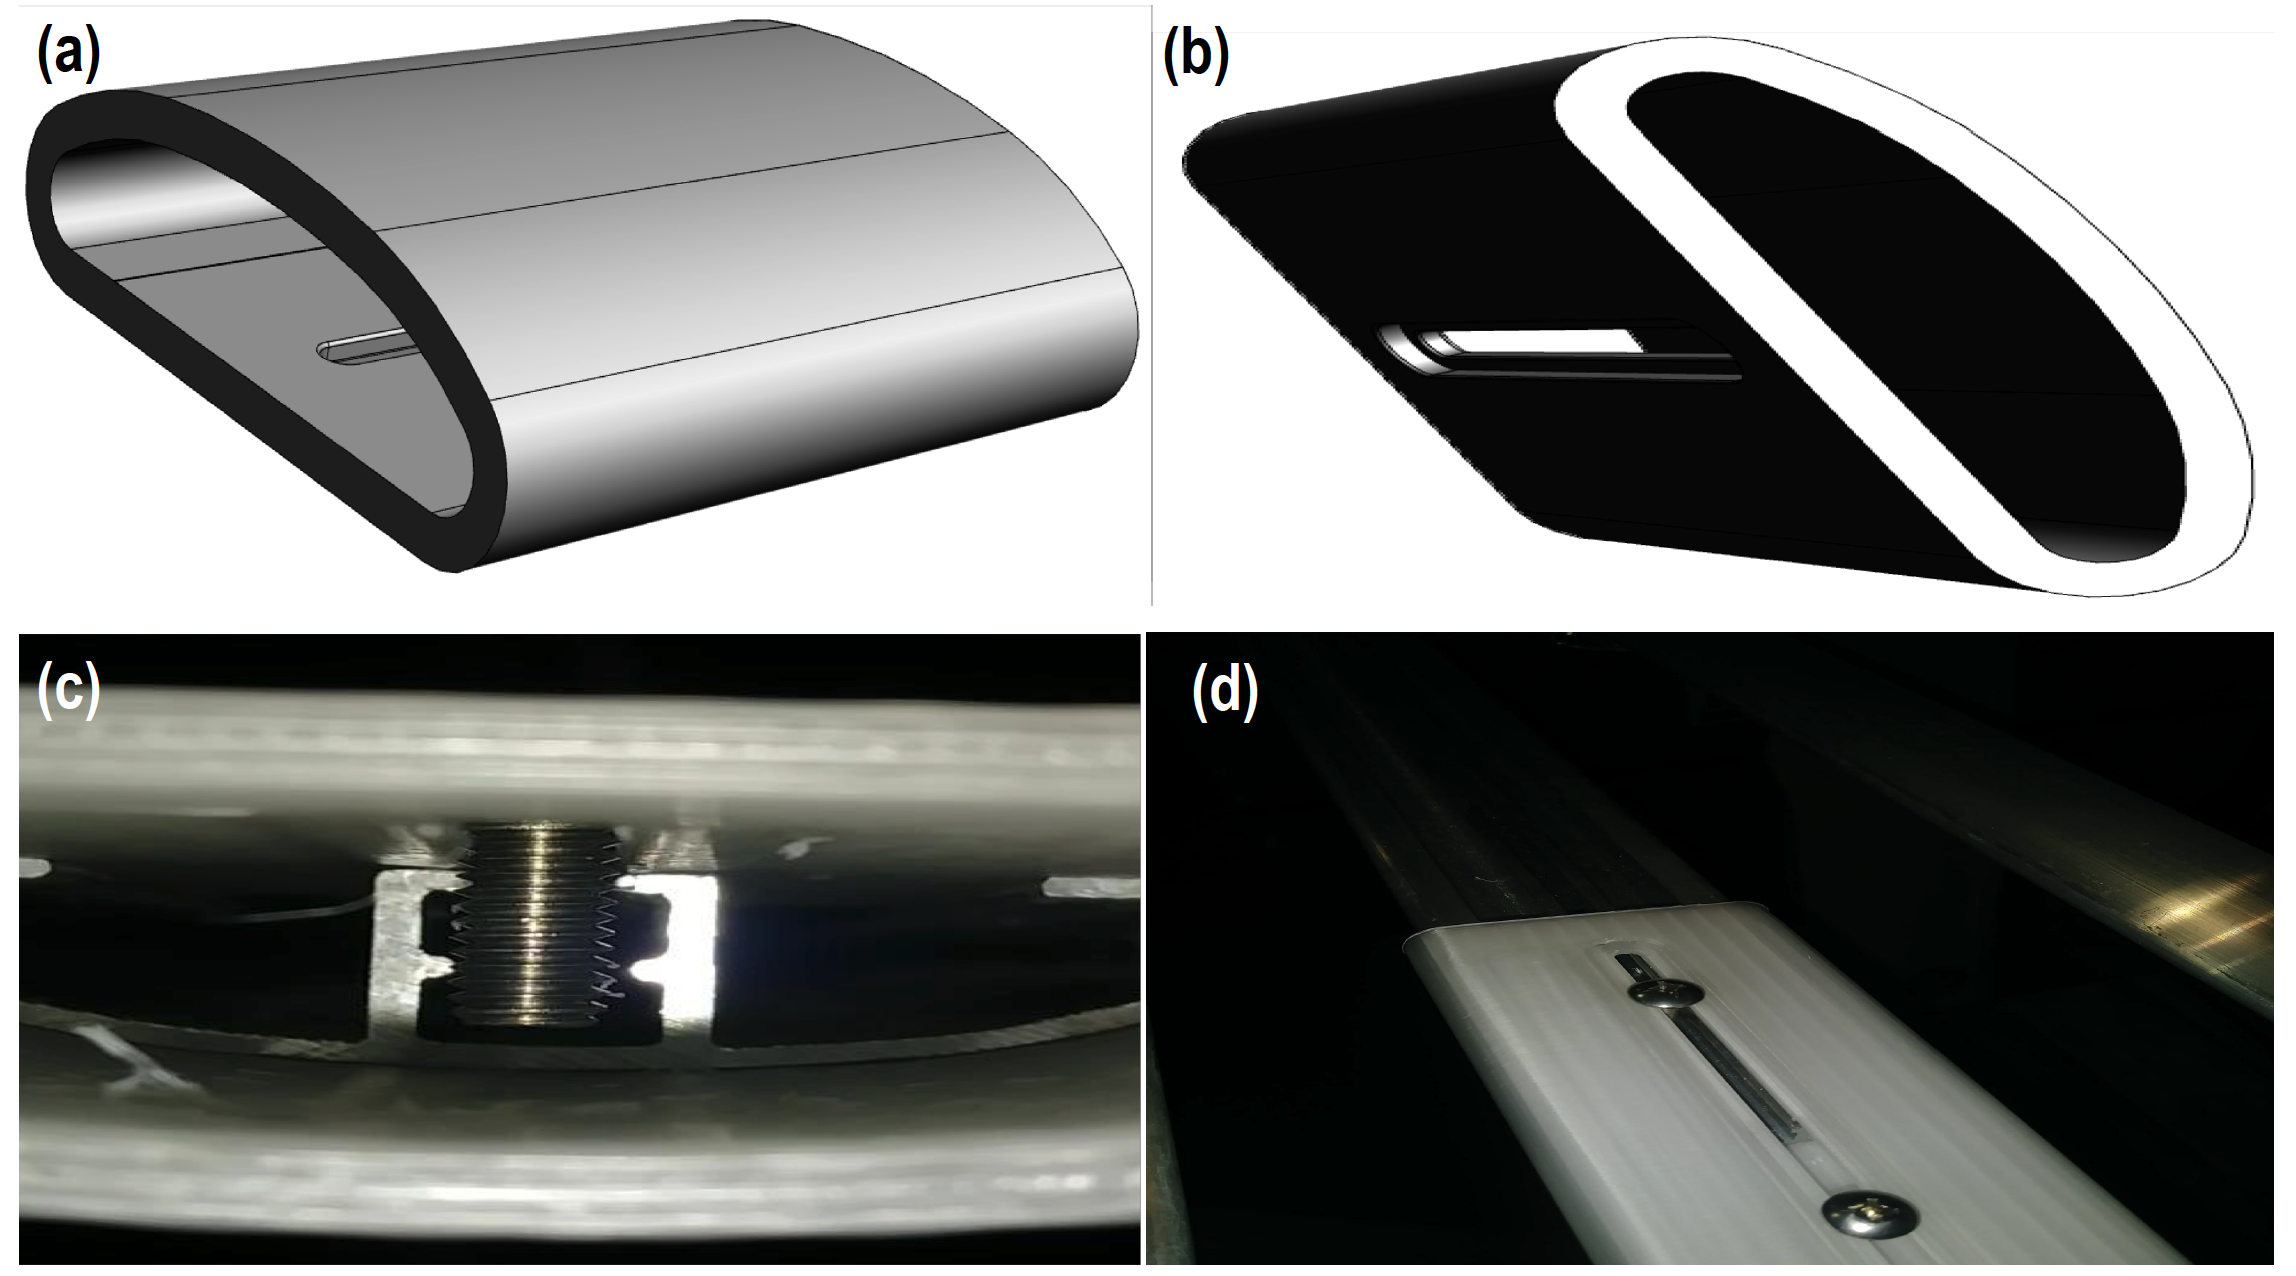
\includegraphics[width=0.8\textwidth]{DP_HVS_FC_Profile_Resistive_Sheath.png}
\end{dunefigure}

A resistive sheath connects the ends of each set of two end-to-end \dword{fc} profiles, as depicted in Figure~\ref{dunefiglabel:resistive-sheath} c and d, forming continuous equipotential rectangular rings  \SI{144}{\m} long. 
\Dwords{hvdb}, consisting of two resistors and a series of four surge-protection varistors in parallel, bridge the gap between the two neighboring stacked profile rings.   The total number of \dword{hvdb} rows will be determined based on redundancy and the limit requirements on current;  one row of \dword{hvdb} is in principle sufficient to provide the required potential difference of \SI{3}{\kV} between neighboring rings, but more are desirable for redundancy.


The resistive chain for voltage division between the profiles provides a linear voltage gradient between the cathode and the top-most field shaping ring. This chain is critical because it determines the strength of the \efield between one profile and its neighbors as well as between the profile and other surrounding parts like the grounded stainless steel membrane. The \efield must be kept well below \SI{30}{\kV\per\cm} at all points in the \lar bath to keep \dword{tpc} operation safe.

Each stage of the \dword{hvdb} consists of two \SI{5}{\giga\ohm} resistors in parallel and two variable resistors of threshold voltage \SI{2}{kV} to protect the resistors in case of a sudden discharge.  With 199 stages under 600kV potential, the total expected current at \dptargetdriftvoltpos is therefore \SI{1.2}{\micro\ampere} per row.  A total of 12 rows, connected in parallel, are used for redundancy in \dword{dpmod}, so the expected current in the entire system is \SI{14.3}{\micro\ampere}.
For optimization, one \dword{dpmod} \dword{hvdb} will connect \num{11} stages.  This means  one \tpcheight tall module can be covered by fifteen \num{11} stage \dword{hvdb} and one \num{10} stage \dword{hvdb} at the bottom to make the final connection.  

Figure~\ref{fig:pddp-hvdb} shows one \dword{pddp} \dword{hvdb} board and  Figure~\ref{fig:dune-dp-fc-all} d shows the connection of one row of \dword{hvdb} along the entire height of the \dword{fc} as installed in \dword{pddp}. The \dptpcwdth (W) $\times$ \dptpclen (L) ground plane consists of \num{80} unit planes (each \SI{3}{\m} $\times$ \SI{3}{\m}).  

The cathode plane is mounted to the bottom of the \dword{fc}, together forming one contiguous unit of field-providing structure.  The bottom-most \dword{hvdb} makes the connection between the cathode and the bottom-most field-shaping ring.
For redundancy, a total of two \dword{hvdb} rows are used in \dword{pddp}.  
The \dpmod will use one \dword{hvdb} chain every four \dword{fc} modules, providing ample redundancy.  However, the final number of rows of \dword{hvdb} must take into account the impact of the underlying current through the \dword{fc} due to particle interactions.

\subsection{HV Return and Monitoring Devices}

To maintain the potential difference between the top-most field shaping ring and the extraction grid of the charge readout plane, either a dedicated \dword{hv} supply and an adjustable resistor chain is used in the \dword{hv} return outside of the cryostat. \fixme{The previous sentence needs some clarification. Either requires an or, but in this sentence, we have either/and. Do you need both the HV supply and the resistor chain? Or is it one or the other, but not both?}  This requires an independent \SI{10}{kV} \fdth similar to those developed for the extraction grid.

Several devices will monitor the \dword{hv}:  
\begin{itemize}
\item The Heinzinger units have typical sensitivities down to tens of nanoamperes with current readback capability.  The units can sample the current and voltage every few \SI{100}{\milli\s}.  
\item Inside the cryostat, so-called pick-off points near the anode will monitor the current through the \dword{hvdb} resistor chain. Additional pick-off points could be implemented on the \dword{gg} below the cathode to monitor possible stray currents.
\end{itemize}


\section{Quality Assurance and Quality Control}
\label{sec:fddp-hv-qa}

\subsection{Field Cage} When FRP I-beams and other parts are delivered, they all undergo a visual inspection to look for defects, in particular those affecting structural integrity, such as cracks, air bubble holes, depression, and flatness. The parts are sorted into three preliminary categories: category 0 (pass), category 1 (problematic but could be repairable), and category 2 (severe and unusable) .

The visual inspection is followed by critical dimension measurements to verify individual sub-module assembly and module interconnection integrity.  These measurements focus on cross sectional dimensions for rods, plates, and bars, as well as length, straightness, flatness, and camber of the beams and flanges.
All measurements must satisfy the mechanical tolerance provided by the design drawings and the standard industry quality criteria.

The FRP I-beams and parts in category 1 undergo a repair process during the preparation stage through defibering, deburring, and sanding.  Another set of measurements is performed after the repair to redetermine the part's category.

Those in category 2 are returned to the vendor for replacement.

All FRP parts that pass inspection are prepared for use, which involves \dword{qc} at each step.  Each part is first defibered, deburred, sanded to smooth the edges, then varnished to
suppress any remaining fibers.  Once the part is prepared, it is stored in a humidity and temperature controlled drying area for \numrange{24}{48} hours to fully cure the varnish.  After full curing, each module is laser-engraved with a unique part number and recorded in a \dword{qc}  database. 

At this point, the sub-module is pre-assembled on a table before packaging to ensure all parts fit, including inserts, screws, and slip nuts.   When fitness is verified, the sub-module is disassembled and packaged in a \SI{10}{\cm}$\times$\SI{10}{\cm}$\times$\SI{2}{\m} compact package and the edges wrapped with a thick plastic layer to protect the parts from mechanical damage from falls or other accidents.  This package includes all necessary parts to assemble the given sub-module along with \numrange{10}{20}\% spare parts.  This ensures that each package is self-sufficient for final assembly.  Each package is given a sub-module number for further tracking.  This sub-module number stays with it throughout assembly at \surf and final installation, so the sub-module can be assigned to its specific module and to its proper location within the module. 

%%%%%%%%%%%%%%%%%%%%%%%%%%%%
\subsection{Electrical Interconnections and HV Divider - 1.5 pages}
\label{sec:fddp-hv-prod-interconnect}

A resistive sheath connects the ends of each set of two end-to-end \dword{fc} profiles, as depicted in Figure~\ref{dunefiglabel:resistive-sheath} c and d, forming continuous equipotential rectangular rings  \SI{144}{\m} long. 
\Dwords{hvdb}, consisting of two resistors and a series of four surge-protection varistors in parallel, bridge the gap between two neighboring stacked profile rings.   The total number of \dword{hvdb} rows will be determined by redundancy and current limit requirements;  one row of \dword{hvdb} is in principle sufficient to provide the required potential difference of \SI{3}{\kV} between neighboring rings, but more are desirable for redundancy.


The resistive chain for voltage division between the profiles provides a linear voltage gradient between the cathode and the top-most field shaping ring, which is critical because it determines the strength of the \efield between one profile and its neighbors, as well as between the profile and other surrounding parts like the grounded stainless steel membrane. The \efield needs to be kept well below \SI{30}{\kV\per\cm} at all points in the \lar bath to keep \dword{tpc} operation safe.


Two distinct types of \dword{hv} divider boards are used for \dword{pddp}: \num{10} and \num{8} stage boards.  Each stage consists of two \SI{2}{\giga\ohm} resistors in parallel and four variable resistors with a threshold voltage of \SI{1.28}{kV} to protect the resistors in case of a sudden discharge.  The total expected current at \dptargetdriftvoltpos is therefore \SI{3}{\micro\ampere} per row.  Several rows, connected in parallel, are used for redundancy, so the expected current in the entire system is simply the number of rows times the current for each row.
For optimization, one \dword{dpmod} \dword{hvdb} will connect \num{11} stages.  This allows  one \tpcheight tall module to be covered by fifteen \num{11} stage \dwords{hvdb} and one \num{10} stage \dword{hvdb} at the bottom to make the final connection.  

Figure~\ref{fig:pddp-hvdb} shows one \dword{pddp} \dword{hvdb} board and  Figure~\ref{fig:dune-dp-fc-all} d shows the connection of one row of \dwords{hvdb} along the entire height of the \dword{fc} as installed in \dword{pddp}. The \dptpcwdth (W) $\times$ \dptpclen (L) ground plane consists of \num{80} unit planes (each \SI{3}{\m} $\times$ \SI{3}{\m}).  
The cathode plane is mounted to the bottom of the \dword{fc}, together forming one contiguous unit of field-providing structure.  The bottom-most \dword{hvdb} makes the connection between the cathode and the bottom-most field-shaping ring.
For redundancy, two \dword{hvdb} rows are used in \dword{pddp}.  
The \dpmod will use one \dword{hvdb} chain for every four \dword{fc} modules, providing ample redundancy.  However, the final number of rows of \dwords{hvdb} must take into account the impact of the underlying current through the \dword{fc} due to the particle interactions.

%{\bf \dword{hv} Divider Board}
%All resistors used for board production are numbered and undergo a three-step quality test for final selection; (1) room temperature resistance measurement at voltages up to \SI{4}{kV} in \SI{500}{V} steps; (2) LN resistance measurement at voltages up to \SI{4}{kV} in \SI{500}{V} steps; and (3) resistance measurements at voltages up to \SI{4}{kV} in \SI{500}{V} steps after warming up to room temperature.  Once the resistance of all resistors is measured, the measured values are histogrammed for the final selection.   
All resistors used for board production are numbered and undergo a three-stage \dword{qa} test for final selection. Resistance is measured at voltages up to \SI{4}{kV} in \SI{500}{V} steps for each stage. The first stage of testing is done at  room temperature, the second at LN temperature, and the third again at room temperature after warming up.  The measured values are histogrammed for final selection to look for groupings of values.   
%The selection is made based on the grouping of the resistors whose resistance are within 1\$ of each other using the results from all three testing stages.   
%It is more important to have the resistance values close to each other than being the given value (unless they are totally out of range from the design values) selecting the tighter grouping provide better quality assurance.
It is more important that the resistance values be close to each other than that they be at any particular value (unless they are too far from the design values). The resistors for which the resistance values are within 1\$ \fixme{This shows up on the PDF as 1 dollar. I do not think that is correct.} of each other are selected.   \fixme{I reworded the prev paragraph}

All varistors for board production are also numbered for \dword{qa} purposes and undergo a three-stage \dword{qa} testing program for the final selection. Each test stage is a clamping voltage measurement, first at room temperature, then at LN temperature, and again after warming back up to room temperature.  
The measured values are histogrammed for final selection; those for which the clamping voltage is closer to the design values are selected to ensure proper protection.   

Once the electrical parts are mounted on the \dword{hvdb} by the vendor, they undergo a three-stage \dword{qa} testing program. Each stage involves a resistance measurement, first at room temperature, then at LN temperature, and again after warming back up to room temperature.  The measured values are histogrammed for the final selection.
The boards can fall into one of three categories: 0. Pass, 1. Repairable, and 2. Rejected.  
If at any testing stage the resistance is more than \SI{0.5}{\%} away from the mean, the part does not fall into category 0, pass.  Boards in category 1 are sent back to the vendor with the selected resistors, so the parts in failed stages can be replaced with the resistors selected during the resistor tests. %\fixme{with the selected resistors? pls clarify}

{\bf Aluminum Profiles and Resistive Sheath:}
The \dword{qa} testing of the aluminum profiles and the resistive sheath is done on prototype production samples before full production begins.   The samples are visually inspected for shape and adherence to the design drawing and for surface smoothness, surface-coating quality, and smoothness of the bend (for profiles with the \num{90}$^{\circ}$ bend).  The resistive sheath samples are visually inspected for shape and adherence to the drawing, edge smoothness, and mechanical fitness, as well as how tightly they fit to the profiles while still allowing an easy slide to couple to the neighboring profile.

{\bf Power Supply and Feedthrough:} The power supply is tested extensively along with the controls and monitoring software.  %Features to be included in the software \fixme{tests?} are:
Capabilities to test include
\begin{itemize}
\item Ramp and change the voltage, including rate change and pause capabilities and settings; 
\item Accept user-defined current limit:  This parameter sets the value of current at which the supply reduces the voltage output to stay below it.  The current limiting itself is done in hardware;
\item Accept a setting for the trip threshold current:  At this threshold, the software would reduce the voltage output. 
In previous experiments, the trip function in software would set the output to \SI{0}{kV}; 
\item Record the current and voltage readback values with a user-defined frequency and record any irregular current or voltage events. 
\end{itemize}


\subsection{Quality Control - 2 pages}
\label{sec:fddp-hv-transport-QC}
Assembly, testing, transportation, and installation procedures must ensure adequate \dword{qc} of all \dword{hv} system components.% are being defined, tested and documented during the construction of \dword{pddp}.

The \dword{fc} sub-modules are assembled inside the cryostat on an assembly table with a precision alignment bar.%, as in \dword{pddp}.  %A sub-module FRP part package will be visually inspected for any external damages and will be opened carefully to avoid any damage to the FRP parts.  
Each sub-module-FRP part package is visually inspected for external damage and is opened carefully to avoid damage to the FRP parts.  
Bags of hardware are removed and set side. The two \SI{10.2}{\cm} (\SI{4}\,in) I-beams, two stainless steel cross bar tubes with diameters of \SI{2.5}{cm} (\SI{1}{in}), and connecting L-brackets are visually inspected for  damage incurred during transport.  Once the FRP parts pass inspection, they are assembled into the frame on the table.  

The aluminum profiles are visually inspected and felt by hand for severe scratches and sharp points.  The profiles that pass are inserted into the profile slots on the FRP sub-module frame, with one fixing slip nut inserted into the rail on the reinforcement rip, 
\fixme{what is this?} Assembly and alignment follow the process described in Section~\ref{sec:fddp-hv-prod-assy-fc-frames}.  The alignment of the profiles is checked using a straight-edge along one end of the profile.  The sub-modules that pass are put on the wheel base and stored until they can be installed.

The \dword{hv} divider boards are tested on-site for resistance of each stage at room temperature to ensure the integrity of the board and the electrical connection of the resistors before installing the boards onto the sub-module. 

At \surf, cathode and \dword{gp} modules are checked for the required planarity and mechanical integrity. In addition, during the installation phase, the electrical continuity between the modules is checked.

The \fdth and the \dword{hv} extender are tested simultaneously at the \dword{itf}, 
\fixme{I replaced: testing facility  site (possibly at CERN) }
preferably with the planned %purchased 
power supply. To pass, the \fdth must hold the goal voltage (\dptargetdriftvoltneg{}) in ultra pure \lar (\dword{tpc}-quality purity corresponding to a free electron lifetime, $\tau\geq$\SI{7}{\ms}) for at least \num{24} hours. The ground tube submersion and \efield environment of the test set up must be comparable to the real \dword{fc} set up or a more challenging environment. Additionally, the \fdth must be UHV-grade leak tight.

Upon arrival at \surf, the power supply used in the \dword{dpmod} \dword{hv} system is tested before installation, with output voltages and currents checked on a known load. 

\noindent 
%%%%%%%%%%%%%%%%%%%%%%%%%%%%
\section{Safety}
In all phases of \dword{hv} system development of the \dpmod, including fabrication, installation, and operations, safety is the highest priority.  As for \dword{pddp}, all assembly, testing, transport, and installation procedures will be documented. Explicit attention is paid to how well \dword{pddp} procedures transfer to the \dpmod. The most critical of these are noted in the preliminary \dword{hv} risk assessment. \fixme{add reference}
\fixme{This section will discuss interaction of HV experts with
Integration team, and reference the appropriate chapter/volume for further details.}

\subsection{Production Safety - 1 page}
\label{sec:fddp-hv-prod-safety}

The \SI{10.2}{\cm} (\SI{4}\,in) \SI{2.0}{\m} long FRP I-beams are delivered with screw holes already drilled to hold aluminum profiles.
These I-beams must be processed to eliminate any remaining fiber or slivers of plastic.
This requires a set process already tested at \dword{pddp} \dword{fc} module production.
Sanding, deburring, and varnishing prepare I-beams, and preassembly verifies the fitness of the parts. 
The \SI{2.54}{\cm} (\SI{1}\,in) \SI{2.0}{\m} long stainless steel cross bars must be filed and sanded to remove chips and slivers.

Personnel participating in the production process will be trained thoroughly with hazards present in the process.  
Care will be taken to avoid personnel overextending as they lift the parts up and to use care in moving parts around. 
Pallet jacks, dollies, and hoist will be used for lifting to avoid any injuries from moving heavy equipment. 
Personnel will be trained using the production site's Back Injury Prevention as a preventive measure.
I-beam and the stainless steel tube manipulation will be done with extreme care to avoid injury to any personnel or damaging any parts or equipment. 
Care will be taken to avoid spilling liquid (ethanol, simple-green, varnish, or de-ionized water) on the floor to prevent slippage. 
Any spilled liquid will be mopped immediately with a floor mop.
All personnel will use gloves, protective glasses, and mask while
working with ethanol, epoxy, and simple green. 
Users will have the appropriate respiratory protections following the production site's Respirator Program rules and receive respirator training as
required.

\subsection{Handling Safety -  1 page}
\label{sec:fddp-hv-transport-safety}
%\subsection{Assembly and Installation}
%\label{sec:fddp-hv-install}

The structural and electrical designs for the \dword{dp} \dword{hv} system are based on designs that are vetted and validated in \dword{pddp} construction, which is currently in its final phase of deployment at CERN. In parallel with the \dword{pddp} construction and operation, \dword{hv} tests at CERN are planned using %foreseen implementing 
full-voltage and full-scale \dword{hv} \fdth, power supply, and monitoring system in dedicated \dword{hv} test facilities. This also provides an opportunity %, allowing also 
to complete full safety reviews. 

Operating the \dword{fc} at its full operating voltage produces a substantial amount of stored energy. The modular design of the cathode specifically addresses this safety concern: in the event of a power supply trip or other failure that unexpectedly drops the \dword{hv}, the charge stored in the segmented cathode structure limits the power dissipated. 
This design will be tested in \dword{pddp} at \SI{300}{kV} voltage over \SI{9}{\m$^2$} surface segmented in four cathode modules.  

Integral to the \dword{dp} \dword{fc} design, both in \dword{pddp} and the \dpmod, is the concept of pre-assembled modular panels of field-shaping conductors with individual voltage divider boards. The structural design and installation procedures used in \dword{pddp} were selected to be compatible with use at the \dword{fd} site and were vetted by project engineers, engineering design review teams, and CERN's safety engineers. Some revisions to these designs are expected based on lessons learned in installation and operations; these revisions will be reviewed both within the \dword{dune} project and by \fnal EH\&S personnel. The overall design is on solid footing. 

Assembly of the \dword{fc} panels and resistor-divider boards involves labor from the collaboration members, technical staff, and students and  does not present unusual industrial hazards. The \dword{hv} consortium will work closely with each assembly site to ensure that procedures meet both \fnal{}'s and institutional requirements for safe procedures, personal protective equipment, environmental protection, %trained 
materials handling, and training. Most %production 
part fabrication will be done commercially and shipping will be contracted through approved commercial shipping companies. Before a site is approved as a production venue, an external safety panel will visit the site for review to ensure best practices are in place and maintained. 


%%%%%%%%%%%%%%%%%%%%%%%%%%%%%%%%%%%%%%%%%%%%%%%%%%%%%%%%%%%%%%%%%%%%
\section{Transport, Assembly, and Installation and Integration}
\label{sec:fddp-hv-transport}

%%%%%%%%%%%%%%%%%%%%%%%%%%%%
\subsection{Transport and Handling - 1 page}
\label{sec:fddp-hv-transport-transport}

The \dword{fc} FRP beams and G10 parts are shipped in a standard wooden crate.  Parts for each sub-module are packed into one %IKEA-style package 
flat pack \SI{0.1}{\m} $\times$ \SI{0.1}{\m} $\times$ \SI{2}{\m} sealed in multiple layers of shrink wrap and a thick, soft cushion of plastic for edge protection. Because each sub-module package is so compact, each wooden crate \SI{1.5}{\m} (H) $\times$ \SI{1.3}{\m} (W) $\times$ \SI{2.5}{\m} (D) can transport 110 sub-module flat pack stacked in 10(W)$\times$11{H} formation.
The total number of sub-module flat packs for the entire \dword{fc} is \num{216}, excluding spares, all \dword{fc} frame parts can be transported in two boxes. 
Each of these crates would weigh less than 2,500kg.
Because the cage for underground transport at \surf is 
\SI{3.6}{\m} (H) $\times$ \SI{1.38}{\m} (W) $\times$ \SI{3.7}{\m} (D) with a load capacity of 13,000 lbs, or approximately 6,000 kg, in principle, all \dword{fc} frame parts can be transported \fixme{...transported where?} in one trip.

The extruded aluminum profiles for \dword{fc} are shipped separately in  standard wooden crates. In all, \num{199} profiles are needed for each \tpcheight module. Therefore, \num{7,164} profiles must be transported underground, excluding spares. The same number of resistive sheaths are also shipped separately in standard wooden crates and transported underground. 

The trusses for cathode modules \SI{12}{\m} (L) $\times$ \SI{30}{\cm} (H) $\times$ \SI{2.5}{\cm} (W) are welded off site and shipped to \surf in transport containers. 
The \SI{12}{\m} (L) $\times$ \SI{2.5}{\cm} (D) resistive rods are also constructed off site and shipped in standard wooden boxes.  Given the lack of storage space at the 4850L and the installation procedure, the cathode plane is assembled as each cathode unit arrives at the cavern in its assigned order because the \dword{fc} super-modules are assembled in sequence beginning at the opposite end of the cryostat from the \dword{tco}.

The power supply, \fdth{}s, and \dword{hv} extender are sent to \surf in standard shipping crates. Unwrapping requires clean areas and careful handling. Surfaces can be cleaned with alcohol and allowed to dry.

\subsection{Assembly}
An \dword{fc} sub-module is pre-assembled on a table before packaging to ensure fitness of all parts, including all screws and slip nuts.   When fitness is verified, the sub-module is disassembled and packaged in a \SI{10}{\cm}$\times$\SI{10}{\cm}$\times$\SI{2}{\m} compact package with the edges wrapped in a thick plastic layer to protect the parts from mechanical damage from a fall or some similar accident.  This package includes all necessary parts to assemble the given sub-module along with \numrange{10}{20}\% spare parts.  This ensures that each package is self-sufficient for final assembly.  Each package is given a sub-module number for further tracking.  This number stays with the sub-module throughout assembly at \surf and final installation, so the sub-module can be assigned to its specific module and in its proper location within the module. 

The compact packages of the \dword{dpmod} \dword{fc} parts are shipped to \surf and transported underground for final sub-module assembly prior to the installation.   The \SI{4}{\m} long aluminum profiles are produced and shipped to \surf separately for final assembly.  The final \dword{qc} of the profiles is conducted during sub-module assembly.   Profiles with deep scratches and sharp protrusions that could cause excess charge concentration will be rejected. This process must be done underground at the time of sub-module assembly because of the delicate nature of the coated surface and the smoothness requirement. \fixme{I took out: of the smoothness to meet the local maximum field requirement.}

Sub-modules are assembled inside the \dword{dpmod} cryostat. An assembly table with a precision alignment bar for rapid profile alignment is used for this task.   The package is opened on the table and the mechanical frame is assembled using two \SI{10.2}{\cm} (\SI{4}{in}) FRP I-beams and two \SI{2.5}{\cm} (\SI{1}{in}) diameter stainless steel tubes.

Once the frame is assembled, aluminum profiles are mounted on the flange of the FRP I-beams and secured using two slip nuts and metal screws with one side secured tightly and the other loosely to allow motion due to thermal contraction.  Care must be taken to ensure that the profiles are not scratched during the mounting process. 

When all screws are hand-tightened as much as possible, the final torque is applied using the 12V Dewalt Power Screw Driver torque set at 1.  The final alignment of the profiles is then made by hand, tightening only one or two screws on the tightly secured side as needed.
A wheel base made of unistrut bars is then mounted to the bottom of the sub-module, and the entire unit is placed in a designated area to await installation.   The wheel is clearly labeled with the sub-module number for tracking purposes.

%%%%%%%%%%%%%%%%%%%%%%%%%%%%
\subsection{Installation and Integration -  1 page}
\label{sec:fddp-hv-transport-install}
%\subsection{Installation and Integration}
%\label{sec:fddp-hv-integratio}
All \dword{fc} sub-modules are assembled inside the cryostat on an assembly table, including one resistive sheath on each profile for sub-module interconnections.
Once a sub-module is fully assembled, a transport wheel base will be mounted on it for easy relocation.
When \num{3} top sub-modules, \num{3} bottom sub-modules, and \num{12} middle modules are assembled, the installation of these modules into a super-module begins, starting at the far end of the cryostat from the sub-module assembly area.
The installation sequence for a super-module is as follows:
\begin{enumerate}
    \item Hang a \SI{12}{\m} stainless steel I-beam from two stainless steel cables through the \fdth{}s and raise it to approximately \SI{2.5}{\m} above the temporary floor.
    \item Place three top sub-modules under the stainless steel I-beam, and connect each to the I-beam using two sets of stainless steel brackets, SS screws, lock washers, and stainless steel nuts.  
    \item Slide the resistive sheaths over to make the resistive connections between profiles in two sub-modules. This process will complete one row of the sub-modules for a super-module (as depicted in Figure~\ref{fig:dp-super-module-installation-secuence} a).
    \item Raise the completed top row by approximately \SI{2.5}{\m}, place three middle sub-module under the top row, and connect each of the three middle sub-modules to each top sub-module above using \SI{1}{\cm} thick G-10 connection plates and SS screws and nuts.
    \item Once all middle modules are connected to the corresponding top sub-modules, slide the resistive sheath over to make the electrical connections between the sub-modules (as depicted in Figure~\ref{fig:dp-super-module-installation-secuence} b).
    \item Repeat steps 4 and 5 above four more times to complete the assembly of a super-module (as depicted in Figure~\ref{fig:dp-super-module-installation-secuence} c and d).
\end{enumerate}

\begin{dunefigure}[\dword{fc} super-module installation sequence for \dpmod ]
{fig:dp-super-module-installation-secuence}
{(a) The three top sub-modules are mounted to the \SI{12}{\m} stainless steel I-beam using a set of stainless steel L-brackets.
(b) The three middle sub-modules are mounted to each corresponding top sub-module.
(c) The next set of three middle sub-modules are mounted to each corresponding middle sub-module.
(d) A completed super-module with \SI{12}{\m} (W) $\times$ \SI{12}{\m} (H).}
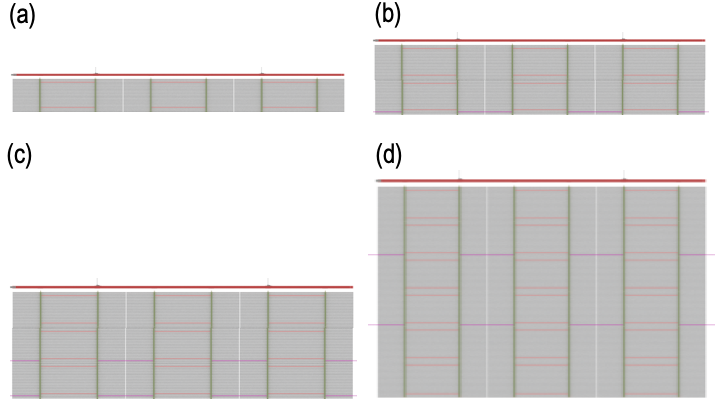
\includegraphics[width=0.9\textwidth]{DP_HVS_FC_super_module_installation_sequence.png}
\end{dunefigure}

The entire \dword{fc}, cathode, ground grid, and photon detector system installation will be done in the following sequence.
\begin{enumerate}
    \item The \endwall super-module with \num{90} degree bent profiles in the far end of the cryostat from the sub-module assembly area will be constructed first.
    \item Then, a U shaped stainless steel cathode \endwall perimeter tube with $\sim$\SI{50}{\mm} diameter will be mounted at the bottom of the \endwall super-module.
    \item This will then be followed by two super-modules along the side wall immediately next to the \endwall module.  
    \item These side wall super-modules will have resistive sheath pre-inserted into each profile to make the electrical connections to the \endwall super-module.
    \item Once the two side wall super-modules are completed, the \endwall super-module with the cathode perimeter tube will then be pulled in \SI{50}{\cm} from its free hanging position, aligned to the side wall super-modules on each side wall and anchored to the temporary floor. 
    \item The \endwall super-module and side wall super-modules are then electrically connected using the pre-inserted resistive sheath.
    \item A cathode module \SI{4}{\m} (W) $\times$ \SI{12}{\m} (L) will be then be mounted to the bottom of the one of the three full height modules in each side wall super-module.
    \item The stainless steel perimeter cathode tube already mounted on the \endwall super-module will then be connected to the corresponding cathode tubes on the side wall super-modules and anchored to the false floor to ensure the mechanical stability of the \endwall super-module until the entire \dword{fc} is constructed.
    \item The temporary floor is removed, and the membrane floor is cleaned.
    \item Ground grids with extended legs are placed under the cathode plane.
    \item The photon detectors that cover the corresponding area will be installed.
    \item The ground grids will be lowered to their nominal height by removing their leg extensions.
    \item Steps 7 - 11 will be repeated one more time to install the cathode, \dword{gg}, and the photon detector to cover two \SI{4}{\m} wide modules from the end.
    \item Two additional side wall super-modules will be constructed and electrically connected to the existing side wall super-modules via resistive sheaths.
    \item Steps 7 - 11 will be repeated three times to cover the \SI{12}{\m} width of the \dword{fc}.
    \item Steps 7 - 13 will be repeated except for the last \SI{4}{\m} wide module of the side wall super-modules that connect to the \endwall super-module on the opposite end.
    \item Steps 1 - 12 will be carried out one last time.
    \item The \endwall super-module floor anchors are removed.
\end{enumerate}

%\clearpage
%\section{Organization and Management}
%\label{sec:fddp-hv-org}

%%%%%%%%%%%%%%%%%%%%%%%%%%%%

%\subsection{Institutional Responsibilities - 1 page}
%\label{sec:fddp-hv-org-consortium}
%%%%%%%%%%%%%%%%%%%%%%%%%%%%
\subsection{Risks - 1 page}
\label{sec:fddp-hv-org-risk-1pg}

%\fixme{Some text must accompany the table. The "ID" in the table refers to the ID in the Risk Register.}
%Most of t
The items presented in %the Risk Table 
Table~\ref{tab:dpHVrisks} apply to %are the same in 
\dword{pddp} and the \dword{dpmod}, and have been addressed by \dword{pddp}, other than %ID's 
items 10, 11, and 14; they are specific to the %Far Detector Underground Installation
\dwords{detmodule}. None %of these items 
have caused significant problems during the commissioning and early operation of \dword{pddp}, with the partial exception of  %ID 
item 6. Current streams occurring at intervals of several hours and localized on one specific \dword{fc} module required a ramp down of the \dword{hv} for a few minutes from the nominal \SI{-600}{kV} to a lower value, unknown at the time of writing this section because the \dword{pddp} has not yet been in operation in \dword{lar}. 
%ID 
Item 5 requires an accurate analysis of collected muon data (this activity is in progress) %( a work-in-progress activity.) 
and the disentangling of space charge effects. 
These risks still persist for the \dwords{detmodule}, %far detector case, 
given the much larger detector scale and the more complex underground installation environment.

\begin{dunetable}
[High Voltage System Risk Summary]
{p{0.15\textwidth}p{0.75\textwidth}}
{tab:dpHVrisks}
{High Voltage System Risk Summary.}   
Item & Risk \\ \toprowrule

1 & Broken resistors on voltage divider boards \\ \colhline
2 & Broken varistors on voltage divider board \\ \colhline
3 & Cathode: Sharp corners at the voltage divider board connections\\ \colhline
4 & Cathode: Truss connections to the field cage\\ \colhline
5 & Angled \endwall super module installation\\ \colhline
6 & Electric field uniformity is not adequate for muon momentum reconstruction \\ \colhline
7 & Electric field is below specification during stable operations\\ \colhline
8 & Damage to \dword{ce} in event of discharge \\ \colhline
9 & Detector components are damaged during shipment to the far site  \\ \colhline
10 & Damages (scratches, bending) to aluminum profiles of Field Cage modules  \\ \colhline
11 & International funding level for DP HVC too low  \\ \colhline
12 & Sole source for Kapton resistive surface; and may go out of production \\ \colhline
13 & Free hanging frames can swing in the fluid flow  \\ \colhline
14 & FPR/Polyethene/laminated Kapton component lifetime is less than expected  \\ \colhline
15 & Underground installation is more labor intensive or slower than expected  \\ 
\end{dunetable}

%\subsection{High-level Cost and Schedule - 2 pages}
%\label{sec:fddp-hv-org-cs}

%\fixme{Cost Summary Table goes in this section.}

%\fixme{Schedule Summary Table goes in this section.}

%\clearpage

%%%%%%%%%%%%%%%%%%%%%%%%%%%%
\section{Interfaces - 1 page}
\label{sec:fddp-hv-transport-interfaces}

\fixme{This section covers mechanical interface to the cryostat, including the penetrations}
\fixme{Interfaces Table goes in this section.}


\subsection{Internal cryogenic system}
\label{sec:fddp-hv-intfc-to-cryogenic}

The interface with the cryogenic system involves the coordination of the placement of the cryogenic pipes. The locations of the ground grid feet, and the \dwords{pmt} must clear the cryogenic pipes on the floor. As of this writing, the nominal position of the vertical gas purging pipe is very close to the \dword{fc} wall.


\subsection{Cryostat}
\label{sec:fddp-hv-intfc-to-cryostat}

The cathode and \dword{fc} are suspended under the cryostat roof through special \fdth{}s. The \dword{hv} \fdth requires a port on the cryostat at a specific location.  The locations, size, height, and load bearing capability of these roof penetrations are being coordinated to allow detailed design of the \dword{hvs}.

%Each \dword{fc} module is suspended and raised by two ropes hung from the cryostat roof through the \dword{fc} suspension \fdth{}s, by winches as in \dword{pddp}.  

%Once an \dword{fc} module of the full height is completed for \dword{dpmod}, it will be hung  from the cables attached to the final suspension hook and the  suspension \fdth is then fully sealed. 

%A possible improvement on the \dword{pddp} interface is to use remote-controlled electrical wrenches (as opposed to manual) to ensure synchronized lifting of the modules.

%%%%%%%%%%%%%%%%%%%%%%%%%%%%%%%%%
\subsection{Charge Readout Plane}
\label{sec:fddp-hv-intfc-to-crp}

These two systems are independently suspended and do not physically touch each other.  The relative vertical position between the top \dword{fc} profiles and the \dword{crp} affects the drift field uniformity near the \dword{crp}.  The \dword{crp}  dynamically follows the liquid surface while the height of the \dword{hvs} is fixed, so the maximum excursion of the \dword{crp}/liquid level must be controlled to avoid excess drift and extraction field distortion.

The \dword{hv} feedthrough and extender structure goes through a corner of the \dword{crp}.  A special \dword{crp} module must be constructed to allow the \dword{hv} feedthrough to be installed.


%%%%%%%%%%%%%%%%%%%%%%%%%%%%%%%%%
\subsection{Photon Detection System}
\label{sec:fddp-hv-intfc-to-pds}

No direct hardware interface exists between the \dword{hv} and \dword{pd} systems. The cryostat penetrations and \fdth{}s for the two systems are completely independent, as are their control electronics. The only interfaces envisaged are effectively at the level of design requirements and include 
\begin{itemize}
    \item maintaining a safe minimum distance between the \dwords{pd} and the \dptargetdriftvoltneg cathode;
    \item defining a mutually agreed upon optical transparency of the cathode + ground grid combination.  In general, a more open cathode/ground grid has higher electric field;
    \item  defining the \dword{pd} power dissipation limit (production of bubbles would compromise \dword{hv} stability). The power dissipation depends on the final \dword{pd} density chosen, which is awaiting simulation results;
    \item if the \dword{pds} wants to install reflector foils on the \dword{fc}, \dword{hvs} is to design a mounting feature for the reflector foils;
    \item installing individual \dwords{gg} on the \dword{pmt} supports in under discussion with the \dword{pds}.
\end{itemize}


\subsection{Slow Control}
\label{sec:fddp-hv-intfc-to-cisc}

The \dword{hvs} relies on \dword{cisc} to control the high voltage power supply and monitor the return currents from the \dword{fc} power return circuits.  An interlock of the \dword{hv} power supply with the liquid level should be implemented to prevent \dword{hv} discharge in gaseous argon.  A controlled shutdown of the \dword{hv} power supply with the opening of the cryostat pressure relief valve must also be implemented.

\subsection{TC}
\label{sec:fddp-hv-intfc-to-tc}

The shipping, storage, underground transportation, assembly, and installation of all \dword{hvs} components are coordinated with technical coordination.


\clearpage
%%%%%%%%%%%%%%%%%%%%%%%%%%%%%%%%%%%%%%%%%%%%%%%%%%%%%%%%%%%%%%%%%%%%

\section{Appendix - Alternatives - 1 page}

\subsection{Optical Reflectors on \dword{fc} FRP Frames}

The \dual \dword{pds} has expressed interest in adding \dword{wls} coated reflector foils on the \dword{fc} inner surfaces to increase light collection efficiency for the upper portion of the \dword{tpc}.  

The reflector foils on their own are very thin and fragile, with different CTE than the rest of the \dword{fc} structure. Unsupported large sheets, therefore, should not be mounted directly onto the \dword{fc}.  However, laminating the reflector foil over a G10/FR4 sheet creates a panel that could be easily attached over the \dword{fc} I-beams.  Because the G10 sheet has a lower CTE than the \dword{fc} profiles, some sliding motion on the mounting fixture should be envisioned.

If the area coverage required is less than \num{50}~\%, the reflector foils may be cut into strips and  installed onto each of the \dword{fc} profiles without any interference with the liquid flow.

The effect of the reflector panels, if their coverage is high, on the \dword{lar} flow pattern and the force exerted on the panels must be studied if this option is chosen.

\subsection{Calibration Laser Penetrations}

Despite being in an underground environment, the \dual detector should have non-neglegible space charge distortion due to the ion feedback from the multiplication of $^{39}$Ar ionizations through the \dwords{lem}. The liquid argon convective flow will make the space charge density distribution difficult to model accurately. Therefore, using UV laser beams is highly desirable to calibrate the charge signal based on the measured field distortions throughout the \dword{tpc} volume.

We have designed a \SI{15}{\cm} offset between the \dword{fc} and the edges of the \dword{crp}, so we may be able to place laser heads through this gap to scan the \dword{tpc} active volume. Obviously, the \dword{fc} support I-beam is in the way, but it should be fairly straightforward to make openings through the I-beam to allow a $\sim $ \SI{10}{\cm} OD object through. This feature will be designed and developed if the calibration consortium decides to implement a laser system.  Naturally, the penetrations for the lasers must be planned in the cryostat design if such a system is likely.



%%%%%%%%%%%%%%%%%%%%%%%%%%%%%%%%%%%%%%%%%%%%%%%%%%%%%%%%%%%%%%%%%%%%
%\section{Installation, Integration and Commissioning}
%\label{sec:fddp-hv-install}
%\fixme{this is kind of mixed up with the next section -anne}

%%%%%%%%%%%%%%%%%%%%%%%%%%%%%%%%%%%%%%%%%%%%%%%%%%%%%%%%%%%%%%%%%%%%
\section{Organization and Management}
\label{sec:fddp-hv-org}

%%%%%%%%%%%%%%%%%%%%%%%%%%%%%%%%%%%
\subsection{HV Consortium Organization}
\label{sec:fddp-hv-org-consortium}

The \dword{hvs} consortium has consolidated all the institutions participating in the design, construction, and assembly of the \dword{hv} systems for both \dword{pdsp}  and \dword{pddp}. 
%
%The consortium 
It currently comprises several USA institutions and CERN, %presently 
the only non-USA participant. As %in the case of 
for \dword{protodune}, CERN is heavily committed to a significant role in terms of funding, personnel, 
 and providing infrastructure for R\&D and detector optimization. Moreover, CERN will be responsible for a significant fraction of subsystem deliverables; as such,  CERN is actively in search of additional European institutions to join the consortium. 
 
 In the \dword{hv} current consortium organization, each institution naturally assumes the same responsibilities that it assumed for %the developments of 
\dword{pdsp} and \dword{pddp}.

The %present 
consortium organizational structure includes a scientific lead from CERN, a technical lead from BNL and, or as fpr the \dword{pddp}, a \dword{tdr} editor from UTA.  \dword{hvs} design and integration  is presently lead at  CERN. 
%  \fixme{structure or leadership? Anne. Refrased: FP}

%\fixme{I removed all the "currently"s -- it's the current consortium org. anne}
 The consortium is organized into working groups addressing the design and  R\&D phases, as well as producing and installing the hardware.

\begin{itemize}
\item WG1. Design optimization for \dword{spmod} and \dword{dpmod}; assembly, system integration, detector simulation, physics requirements for monitoring and calibrations. %Conveners: Jeff Nelson, Vic Guarino, Bo Yu
\item WG2. R\&D activities, R\&D facilities. %Conveners: Francesco Pietropaolo, Ting Miao
\item WG3. \dword{sp}-\dword{cpa}: Procuring resistive panels, frame strips, and electrical connections of planes; assembly, \dword{qc} at all stages, and shipping these parts. %Convener: Stephen Magill
%\fixme{too many QC's. And confusing. Procurement, assembly, QC at all stages, and shipment of these parts? Anne - Done RKP}
%\fixme{Not sure where this came from - do you want detailed list of duties or should it just be the name of the group? - SRM; Simplified: FP}
\item WG4. \dword{dp} cathode and ground plane:  procuring material; construction, assembly, shipping to ITF, \dword{qa}, \dword{qc}.% Convener: Jae Yu
\item WG5.  modules: \dword{sp}-Top/Bottom-\dword{fc} module, \dword{sp}-\endwall modules, \dword{dp}-\dword{fc} modules: procurement of mechanical and electrical components, assembly and shipping to ITF. %Conveners: Thomas Kutter, Michael Wilking, Jeff Nelson, Jae Yu
%\fixme{ditto. Anne}
\item WG6. \dword{hv} supply and filtering, \dword{hv} power supply and cable procurement, R\&D tests, filtering and receptacle design and tests. %Conveners: Franco Sergiampietri, Sarah Lockwitz
\end{itemize}

%Merging of \dword{sp} and \dword{dp} activities is performed for the working groups where synergies have been identified: 
Taking advantage of identified synergies, some activities of the \dword{sp} and \dword{dp} working groups are merged: \dword{hv} feedthroughs, voltage dividers, aluminum profiles, FRP beams, and assembly infrastructure.

\begin{dunetable}
[Participating institutes]
{p{0.15\textwidth}p{0.75\textwidth}}
{tab:instit}
{Institutes Participating in the HVS Consortium.}   
Item & Institution \\ \toprowrule%(Contact, E-mail) 

1 & CERN, Switzerland \\ \colhline%(Francesco Pietropaolo; francesco.pietropaolo@cern.ch) 
2 & Argonne National Lab, USA \\ \colhline%(Steve Magill; srm@anl.gov) 
3 & Brookhaven National Lab, USA \\ \colhline%(Bo Yu; yubo@bnl.gov) 
4 & University of California Berkley / LBNL, USA \\ \colhline%(Cheng Ju Lin; cjslin@lbl.gov)
5 & University of California Davis, USA \\ \colhline%(Emilja Pantic; pantic@ucdevis.edu) 
6 & Fermi National Accleratior Lab, USA \\ \colhline%(Sarah Lockwitz; lockwitz@fnal.gov) 
7 & University of Houston, USA \\ \colhline%(Andrew Renshaw; arenshaw@central.uh.edu) 
8 & Kansas State University, USA \\ \colhline%(Glenn Horton-Smith; gahs@ksu.edu)
9 & Louisiana State University, USA \\ \colhline%(Thomas Kutter; kutter@phys.lsu.edu) 
%10 & South Dakota School of Mines and technology, USA (Juergen Reichenbacher; Juergen.Reichenbacher@sdsmt.edu) 
10 & SUNY Stony Brook, USA \\ \colhline%(Michael Wilking; michael.wilking@stonybrook.edu) 
11 & University of Texas Arlington, USA \\ \colhline%(Jaehoon Yu; jaehoonuy1@gmail.com) 
12 & Virginia Tech, USA \\ \colhline %(Jon Link; jmlink@vt.edu) 
13 & College of William and Mary, USA \\ %(Jeff Nelson; jknels@wm.edu)  
\end{dunetable}

At present, the \dword{hv} consortium is gathering %together all the institutions that are participating 
institutions to participate in the design, construction, and assembly of the \dword{hv} systems for both \dwords{spmod} and \dwords{dpmod}. %There is still the need to expand this list in the near future with effort in including new EU participants.
The consortium is likely to expand in the near future. Discussions are underway with institutions, in particular from EU, to balance USA participation with additional international partners.




%%%%%%%%%%%%%%%%%%%%%%%%%%%%%%%%%%
\subsection{Planning Assumptions}
\label{sec:fddp-hv-org-assmp}

The present baseline design for all elements of the \dword{hv} system for \dword{dpmod} follows the experience with \dword{pddp} as well as the \dword{pdsp} designs including production and assembly.  

It is also assumed that no major issues in the \dword{hv} system operation of \dword{pddp} will be encountered, and therefore the basic \dword{hv} system concepts are sound.

However some design modifications and optimizations have been implemented to take into account the %twice-as-long 
doubled drift distance, indicating an increase in \dword{hv} delivery to the cathode from \SI{-300}{\kV} to \dptargetdriftvoltneg{} and the much higher energy stored in the cryostat because of the applied \dword{hv}.

Therefore the \dual \dword{hv} system distribution and the related cathode structure still require intense R\&D, given the unprecedented value of the required \dword{hv} (\dptargetdriftvoltneg).
The related results could lead to revising design details such as the shape of the cathode elements and of the %\dword{gg} 
\dword{gp} structures, the distance from the cryostat walls, the distance between the cathode and the %\dword{gg} 
\dword{gp} protecting the \dwords{pd}, and resistive connections of the cathode modules. We must ensure that the \efield intensity in the \lar is below the critical value of  about \SI{30}{\kV/\cm} everywhere and that the energy stored in the \dword{fc} is not released catastrophically to the detector membrane. % skin.

As for the \dword{spmod}, \dword{pddp} will be the playground where we come to understand and optimize detector element assembly, installation sequence, and integration as well as requirements in %manpower, 
human resources, space and tooling, and schedule. 

%%%%%%%%%%%%%%%%%%%%%%%%%%%%%%%%%%%

\fixme{The editors at meeting of 2/13 suggest that the WBS section should be deleted in the TP. Accordingly, I have commented it out. RKP}

%%%%%%%%%%%%%%%%%%%%%%%%%%%%%%%%%%%
%\subsection{WBS and Responsibilities}
%\label{sec:fddp-hv-org-wbs}
%
%Consortium deliverables and related Working Breakdown Structure have also been derived from those identified for the ProtoDUNE detectors. As already mentioned before, responsibilities have been assigned to the institutions members of the Consortium, according to the experience gained with ProtoDUNE.
%
%\fixme{(Here: table to be extracted for the WBS excel file)}
%
%%%%%%%%%%%%%%%%%%%%%%%%%%%%%%%%%%

\subsection{Risks}
\label{sec:fddp-hv-org-risk}

The items presented in %the Risk Table 
Table~\ref{tab:HVrisks} from the \dword{dpmod} are derived from those that will be addressed in  %are the same in 
\dword{pddp}.  Some of these are also common to \dword{pdsp} and the \dword{spmod} (e.g., 1 and 2). Other  %ID's 
items (from 12 to 15), involving long term stability and funding, are instead specific to the  %Far Detector Underground Installation
\dwords{detmodule}. 

Items common to \dword{pdsp}  have not caused significant problems during commissioning and early operation of \dword{pdsp}, with the partial exception of  %ID 
item 4. For this specific issue, the operation of \dword{pddp} is essential because the \dword{hvs} layout is different, and the absolute voltage on the cathode is much higher. 
%ID 
Item 5 will require an accurate analysis of collected muon data  %( a work-in-progress activity.) 
to disentangle space charge effects. 
These risks still persist for the \dwords{detmodule}, %far detector case, 
given the much larger detector scale and the more complex underground installation environment.


\begin{dunetable}
[DP High Voltage System Risk Summary]
{p{0.15\textwidth}p{0.75\textwidth}}
{tab:HVrisks}
{High Voltage System Risk Summary.}   
Item & Risk \\ \toprowrule

1 & Broken resistors on voltage divider boards \\ \colhline
2 & Broken varistors on voltage divider board \\ \colhline
3 & Electric field uniformity is not adequate for muon momentum reconstruction \\ \colhline
4 & Electric field is below specification during stable operations\\ \colhline
5 & Space front from positive ions distorting the E field beyond expectation \\ \colhline
6 & Damage to \dword{ce} in event of discharge \\ \colhline
7 & Energy stored in \dword{fc} (in DP) is suddenly discharged.   \\ \colhline
8 & Detector components are damaged during shipment to the far site  \\ \colhline
9 & Damages (scratches, bending) to aluminum profiles of Field Cage modules  \\ \colhline
10 & Bubbles from heat in PMTs or resistors cause HV discharge  \\ \colhline
11 & Free hanging frames can swing in the fluid flow  \\ \colhline
12 & FPR/Polyethene/laminated Kapton component lifetime is less than expected  \\ \colhline
13 & Lack of collaboration effort on this HV system  \\ \colhline
14 & International funding level for DP HVC too low  \\ \colhline
15 & Underground installation is more labor intensive or slower than expected  \\ 
\end{dunetable}



\subsection{High-level Cost and Schedule}
\label{sec:fddp-hv-org-cs}

A first high-level summary of the cost estimate for the \dword{hv} system of one \dword{dpmod} was obtained by extrapolating from the as-realized \dword{pddp} costs and effort, except for the cathode that was introduced as a new concept and whose estimation is more uncertain. Moreover, these estimates do not include any projected cost savings that would be realized by producing many units at each production site. %Given the small numbers of each unit required for the \dword{pddp} the assembly sites were still climbing the learning curve; this could give substantial savings. 
Substantial savings from higher-volume production is still possible, however. For \dword{pddp} the assembly sites produced only small numbers of each unit, and thus remained on the learning curve. 

\begin{dunetable}
[Cost estimates for the \dword{hv} system materials [This table has to be expanded with more details )]
{p{0.40\linewidth}p{0.15\linewidth}p{0.15\linewidth}p{0.15\linewidth}}
{tab:HVcost}
{Cost Estimates for the \dword{hv} System Materials.}   
Element&Unit Cost  (FY18 k\$)& Units per \dword{fd} Module & Total Cost  (FY18 k\$)\\ \toprowrule
cathode plane with resistive elements (\SI{12x4}{\m} unit) &\num{0}&\num{15}&\num{0}\\ \colhline
\dword{gg} plane (\SI{3x3}{\m} unit) &\num{0}&\num{80}&\num{0}\\ \colhline
\dword{fc} sub-module (\SI{4x2}{\m} unit similar to \dword{pddp} but longer profiles)&\num{0}&\num{216}&\num{0}\\ \colhline
\dword{hv} distribution (one power supply + one and one \dword{hv} extender \fdth{}s)&\num{0}&\num{1}&\num{0}\\ \colhline
Total DP1&&&\num{0},\num{0}\\ 
\end{dunetable}

\fixme{(this is to be extracted from the Cost excel file)}
\begin{dunetable}
[\dword{hv} System R\&D Program and Milestones to Lead to CD-2 Approval (THIS TABLE is to be UPDATED in Draft 2)]
{p{0.07\linewidth}p{0.55\linewidth}p{0.10\linewidth}p{0.10\linewidth}p{0.10\linewidth}}
{tab:HVschedule}
{DRAFT- \dword{hv} system R\&D program and milestones to lead to CD-2 approval.}   
WBS&Task Name&Start&Finish \\ \toprowrule
1.5&   CD-2 DOE Review&10/04/19&10/04/19 \\
7& \dword{hv} System& & \\
7.1& Finalize \dual \dword{fc} design&06/27/18&11/30/19 \\
7.2& Finalize \dual cathode design&06/27/18&11/30/19 \\
7.3& Finalize R\&D for 600 kV \dword{hv} \fdth and PS &01/01/18&02/28/19 \\
7.4& Run \dword{dp} \dword{hv} design integration test &02/18/19&02/28/20 \\
7.5& \dword{hv} TDR - Submit for internal review&03/29/19&03/29/19 \\
7.6&\dword{fc} Procurement&  07/08/23& 05/03/24\\
7.7& Cathode and Ground plane Procurement& 07/08/23& 03/04/24\\
7.8& HV distribition procurements (including Voltage dividers)& 09/06/23& 11/29/24\\
7.9& Production readiness reviews& 01/02/24& 01/07/24\\
7.10& Cryostat ready for TPC installation& 08/01/24& 08/01/24 \\
7.11& Cathode and Ground plane assembly& 05/03/24& 12/29/24\\
7.12&\dword{fc} Assembly and installation &08/01/24& 02/03/25\\
7.13& Cathode and Ground plane installation &08/01/24& 02/03/25\\
\end{dunetable}
\fixme{(to do: Schedule)}
